% !TEX encoding = UTF-8 Unicode
% $Header: /cvsroot/latex-beamer/latex-beamer/solutions/generic-talks/generic-ornate-15min-45min.en.tex,v 1.5 2007/01/28 20:48:23 tantau Exp $

%\documentclass{beamer}
\documentclass[10pt]{beamer}
\usepackage[brazil]{babel}
\usepackage[T1]{fontenc}
%\usepackage[latin1]{inputenc}
\usepackage[utf8]{inputenc}
%\usepackage[ruled,linesnumbered,vlined,boxed]{algorithm2e} %pacote para formatar algoritmos

% This file is a solution template for:

% - Giving a talk on some subject.
% - The talk is between 15min and 45min long.
% - Style is ornate.



% Copyright 2004 by Till Tantau <tantau@users.sourceforge.net>.
%
% In principle, this file can be redistributed and/or modified under
% the terms of the GNU Public License, version 2.
%
% However, this file is supposed to be a template to be modified
% for your own needs. For this reason, if you use this file as a
% template and not specifically distribute it as part of a another
% package/program, I grant the extra permission to freely copy and
% modify this file as you see fit and even to delete this copyright
% notice. 


\mode<presentation>
{
  \usetheme{Frankfurt}
  % or ...

  \setbeamercovered{transparent}
  % or whatever (possibly just delete it)
  \setbeamertemplate{theorems}[numbered]
}

%\usepackage[english]{babel}
%\usepackage[brazil]{babel}
% or whatever

%\usepackage[latin1]{inputenc}
% or whatever

\usepackage{times}
%\usepackage[T1]{fontenc}
% Or whatever. Note that the encoding and the font should match. If T1
% does not look nice, try deleting the line with the fontenc.

\usepackage{moreverb} 
\usepackage{verbatim}

\usepackage{hyperref}

\usepackage[ruled,linesnumbered,vlined,boxed]{algorithm2e}

%\usepackage[cmex10]{amsmath}

%\title[Short Paper Title] % (optional, use only with long paper titles)
\title[DEFESA] % (optional, use only with long paper titles)
{Algorithms for the Directed k-Spanner with Minimum Degree Steiner Tree Problem}

%\subtitle
%{Uma solução voltara para reuso e confiabilidade} % (optional)

\author[hugo] % (optional, use only with lots of authors)
{Hugo~Braga}
% - Use the \inst{?} command only if the authors have different
%   affiliation.

\institute[UFBA] % (optional, but mostly needed)
{
  Programa de Pós-Graduação em Mecatrônica\\
  Universidadde Federal da Bahia\\
  Defesa de Mestrado\\
  Orientador: Dr. Flávio Assis}
% - Use the \inst command only if there are several affiliations.
% - Keep it simple, no one is interested in your street address.

\date[Short Occasion] % (optional)
{22 de Outubro de 2012}

\subject{Talks}
% This is only inserted into the PDF information catalog. Can be left
% out. 



% If you have a file called "university-logo-filename.xxx", where xxx
% is a graphic format that can be processed by latex or pdflatex,
% resp., then you can add a logo as follows:

% \pgfdeclareimage[height=0.5cm]{university-logo}{university-logo-filename}
% \logo{\pgfuseimage{university-logo}}



% Delete this, if you do not want the table of contents to pop up at
% the beginning of each subsection:
%\AtBeginSubsection[]
%{
%  \begin{frame}<beamer>{Outline}
 %   \tableofcontents[currentsection,currentsubsection]
 % \end{frame}
%}


% If you wish to uncover everything in a step-wise fashion, uncomment
% the following command: 

%\beamerdefaultoverlayspecification{<+->}
%\newtheorem{lema}[lemma]{Lema}
\newtheorem{lema}{Lema}
\newtheorem{claim}{Afirmação}
\newtheorem{teorema}[theorem]{Teorema}
%\newproof{proof}{Proof}

\begin{document}

\begin{frame}
  \titlepage
\end{frame}

\begin{frame}[allowframebreaks]{Estrutura da apresentação}
  \tableofcontents
  % You might wish to add the option [pausesections]
\end{frame}


% Since this a solution template for a generic talk, very little can
% be said about how it should be structured. However, the talk length
% of between 15min and 45min and the theme suggest that you stick to
% the following rules:  

% - Exactly two or three sections (other than the summary).
% - At *most* three subsections per section.
% - Talk about 30s to 2min per frame. So there should be between about
%   15 and 30 frames, all told.

\section{Motivação}

\begin{frame}{Problema clássico de árvore Steiner}
  \begin{itemize}
  \item O objetivo é encontrar uma árvore que cubra os terminais e que possua custo mínimo.
%  \begin{itemize}
%    \item Entrada:
%      \begin{itemize}
%	\item um grafo $G=(V,E)$, cuja função de custo é representada pela função $C : E \to \mathbb{R}^+$;
%	\item um nó origem $s \in V$;
%	\item um conjunto de terminais $T \subseteq V \setminus \lbrace s \rbrace$.
%      \end{itemize}
%    \item Objetivo: encontrar uma árvore $T_r = (V_{T_r},E_{T_r})$, com nó origem em $s$, que cobre $T$ e possui custo mínimo (i.e. minimiza $\sum_{e \in E_{T_r}} C(e)$).
%  \end{itemize}

%  \item Para um grafo de entrada $G=(V,E)$, cuja função de custo é representada pela função $C : E \to \mathbb{R}^+$, um nó origem $s \in V$ e 
%um conjunto de terminais $T \subseteq V \setminus \lbrace s \rbrace$, o problema clássico de árvore Steiner de custo mínimo pode ser definido como:
%  \begin{itemize}
%    \item Encontrar uma árvore $T_r = (V_{T_r},E_{T_r})$, cujo nó origem é $s$, que cobre $T$ e possui custo mínimo (i.e. minimiza $\sum_{e \in E_{T_r}} C(e)$).
%  \end{itemize}
  \item Aplicada tipicamente na operação de \emph{multicasting}.
  \item Restrições são adicionadas ao problema de \emph{multicasting}:
  \begin{itemize}
    \item Requisitos de Qualide de Serviço (QoS).
    \begin{itemize}
      \item Pode ser modelado através de atraso máximo.
      \item Modelado alternativamente através da propriedade de \emph{spanner}.
    \end{itemize}
    \item Limitação no número de vizinhos da comunicação.
    \begin{itemize}
      \item Restrição de conexões, esforço de replicação de dados, custo de manutenção da topologia em redes móveis.
      \item Pode ser generalizado pela propriedade de limitação do grau máximo.
    \end{itemize}
  \end{itemize}
  \end{itemize}
\end{frame}

\begin{frame}{Outras aplicações}
  % - A title should summarize the slide in an understandable fashion
  %   for anyone how does not follow everything on the slide itself.
  \begin{itemize}
  %\item Árvores Steiner são tipicamente aplicadas na operação de \emph{multicasting}.
  \item Aplicações de \emph{Spanners}:
  \begin{itemize}
    \item Roteamento eficiente.
    \begin{itemize}
      \item Abondanar o requisito de encaminhar mensagens por caminhos de custo mínimo.
    \end{itemize}

    \item Spanners geométricas são utilizadas para diminuir o gasto energético de Redes de Sensores Sem Fio (RSSF).
    \item Utilizadas para aproximar distâncias de custo mínimo.
    \item Utilizadas por oráculos de distância.
  \end{itemize}
  \item Restrições de grau em árvores \emph{Steiner} também existem em cenários onde há a necessidade de balancear a carga na operação de \emph{multicasting}.
  \end{itemize}
\end{frame}

\begin{frame}{Objetivo}
  \begin{itemize}
  \item Buscando modelar o problema de árvore \emph{Steiner} com as restrições de grau máximo e que possua a propriedade de \emph{spanner}, nós procuramos tratar no mestrado 
um novo problema, denominado \emph{Árvore Steiner com Grau Mínimo e fator de dilatação k em Grafos Direcionados} (\emph{Directed k-Spanner with Minimum Degree Steiner Tree Problem} - 
DSMDStP).
  \end{itemize}
\end{frame}

\section{Por quê o problema é novo?}

%\subsection[pequeno titulo]{Motivação}
%\subsection[Motivação]{Motivação}

\begin{frame}{Abordagens anteriores dos problemas de Steiner/Spanner/Grau}
  % - A title should summarize the slide in an understandable fashion
  %   for anyone how does not follow everything on the slide itself.
  \begin{itemize}
  \item Muitos trabalhos assumem espaço euclideano.
  \item Outros trabalhos consideram grafos não-direcionados.
  \item Trabalhos que consideram grafos direcionados:
  \begin{itemize}
    \item Geram árvores geradoras (\emph{Spanning trees}) ou grafos que não necessariamente são árvores.
    \item Tem como objetivo de minização o custo da árvore.
    \item Consideram apenas o requisito de minização do grau.
  \end{itemize}
  \end{itemize}
\end{frame}

\begin{frame}{Trabalhos próximos}
  % - A title should summarize the slide in an understandable fashion
  %   for anyone how does not follow everything on the slide itself.
  \begin{itemize}
    \item \cite{Elkin2009,Elkin2011}:
    \begin{itemize}
      \item Geram \emph{narrow-shallow-low-light trees}.
      \item Resultado final é uma árvore geradora.
      \item Assumem espaço euclideano.
    \end{itemize}
    \item \cite{Elkin2006,Khandekar2011}:
    \begin{itemize}
      \item Problema consistem em gerar árvore \emph{Steiner} que possui grau máximo de saída minimizado em grafos direcionados.
      \item O problema em \cite{Khandekar2011} generaliza o problema abordado em \cite{Elkin2006}, visto que não impõe a restrição de cobrir todo o conjunto de terminais.
      \item Não consideram a propriedade de \emph{spanner}.
      \begin{itemize}
	\item O mais próximo que consideram é limitar a altura da árvore.
      \end{itemize}
      \item A solução para o problema de \emph{Multiple Set-Cover} (MSC) definido pelos autores de \cite{Elkin2006} é base para a nossa solução.
    \end{itemize}
  \end{itemize}
\end{frame}

\section{Formalização do problema}

%\begin{frame}{Definições preliminares}
%  \begin{itemize}
%    \item Algoritmo de aproximação por um fator $\alpha$ \cite{Williamson2011}: consistem em um algoritmo polinomial tal que para todas as instâncias do problema de otimização, 
%produz uma solução cujo valor se aproxima do valor ótimo por um fator $\alpha$.
%    \item Classe de complexidade \emph{DTIME} \cite{Arora2009}: Seja $T : \mathbb{R} \rightarrow \mathbb{R}$ uma função. Uma linguagem $L \in$  \textbf{DTIME}($T(n)$) sse 
%existe uma máquina de Turing que decide $L$ em um tempo de execução de $c \cdot T(n)$, para uma constante $c > 0$.
%  \end{itemize}
%\end{frame}

\begin{frame}{Definição de DSMDStP}
  \begin{itemize}
    \item Entrada:
    \begin{itemize}
      \item Um grafo direcionado $G = (V,E)$, onde o peso de cada aresta é definido por uma função $C: E \rightarrow \mathbb{R}^+$.
      \item Um nó de origem $s$.
      \item Um fator de dilatação $k$ ($k \in \mathbb{R}^+$, $k \ge 1$).
      \item Um conjunto de terminais $T \subseteq V \setminus \lbrace s \rbrace$.
    \end{itemize}
    \item Saída: Encontrar uma arborescência $A=(V_A, E_A)$, com nó origem em $s$ e que cobre $T$, tal que:
    \begin{itemize}
      \item $dist(s,t,A) \le k \cdot dist(s,t,G)$, $\forall t \in T$;
      \item o grau máximo de saída dos nós em $A$, denotado por $D_{max}(A)=max_{v \in V_A}\{odeg(v, A)\}$, é minimizado.
    \end{itemize}
  \end{itemize}
\end{frame}

\begin{frame}{Impossibilidade de aproximação sublogarítmica: \emph{Background}}
  \begin{itemize}
    \item SvMDST é o acrônimo (em inglês) para a versão \emph{Steiner} do problema de Árvore Geradora com Grau Mínimo em Grafos Direcionados \cite{Fraigniaud2001}.
    \begin{itemize}
      \item $T \subseteq V$; $s \in T$.
    \end{itemize}
%    \item Formalmente, SvMDST pode ser descrito como:
%    \begin{itemize}
%      \item Entrada: $G = (V,E)$, $T \subseteq V$ e um nó $s \in T$.
%      \item Saída: arborescência com raiz em $s$ e que cubra $T$, tal que o grau máximo da arborescência seja minimizado.
%    \end{itemize}
    \item A prova da impossibilidade é baseada na redução do DSMDStP para o SvMDST.
  \end{itemize}

  \begin{teorema}
    \label{teorema:steiner_mdst}
    \cite{Fraigniaud2001}
    A menos que $NP \subset DTIME(n^{\log \log{n}})$, a solução ótima para o SvMDST não possui aproximação polinomial por $(1-\varepsilon)\log_e |T|$, para qualquer $\varepsilon > 0$.
  \end{teorema}
  \hyperlink{DTIME_slide}{\beamergotobutton{DTIME}}
  \hypertarget{DTIME}{}
\end{frame}

\begin{frame}{Impossibilidade de aproximação sublogarítmica}
  \begin{claim}
    \label{claim:not_approximable}
    %O problema de Árvore Steiner com Grau Mínimo e fator de dilatação k em Grafos Direcionados (DSMDStP) não admite aproximação polinomial por um fator de
    DSMDStP não admite aproximação polinomial por um fator de 
$(1-\varepsilon)\log_e |T|$, para qualquer $\varepsilon > 0$, a menos que $NP \subset DTIME(n^{\log \log{n}})$.
  \end{claim}
\hypertarget{not_approximable}{}
\hyperlink{not_approximable_slide}{\beamergotobutton{Prova}}
\end{frame}

\section{Algoritmos}

\subsection{APPROX}

\begin{frame}{Algoritmo de aproximação: preliminares}
  \begin{itemize}
    \item <1-> Nosso algoritmo é baseado no algoritmo apresentado em \cite{Elkin2006}. Este foi adaptado para considerar a propriedade de spanner.
    \item <2-> Possui duas fases:
    \begin{itemize}
      \item <3-> fase 1: cômputo da $\sqrt{l}$-partition.
      \item <4-> fase 2: utilização do problema do \emph{Multiple Set-Cover} (MSC) para cobrir os demais terminais.
    \end{itemize}
    \item <5-> $V = C \ \dot \cup U$. Seja $UT = U \cap T$ e $CT = C \cap T$.
    \item <6-> Seja $l = |T|$ e $d^*$ o grau máximo de uma solução ótima para uma instância de DSMDStP ($d^* \leq l$).
    %\item Seja $N(u, G) = \{v : (u, v) \in E\}$. Seja $N(S, G) = \bigcup_{u \in S} N(u, G)$.
    \item <7-> Seja $G(S)$ o grafo induzido por um conjunto de nós $S$.
    \item <8-> Para um nó $u \in U$, $\Delta$-neigh$(u) = \{ t :$ $t \in UT$ $\land$ $dist(s,u,G) + dist(u,t,G(U)) \leq k \cdot dist(s,t,G) \}$.
    %\item Seja $SPT(s, S_{leaves}, G)$ uma árvore formada pela raiz $s$ e caminhos de custo mínimo em $G$ de $s$ para cada nó em $S_{leaves}$.
  \end{itemize}
\end{frame}

\begin{frame}{$\Delta$-\emph{neighbourhood}}
\begin{itemize}
  \item $t = 2$
\end{itemize}

\begin{figure}[H]
\centering
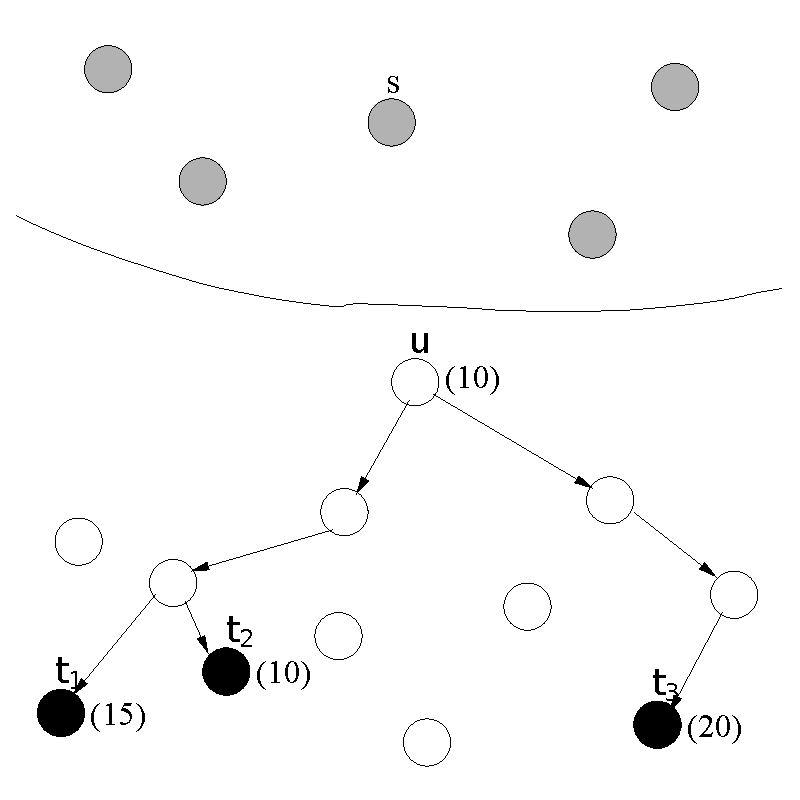
\includegraphics[scale=0.45]{imagens/neigh}
\label{fig:fig}
\end{figure}
%\begin{itemize}
%  \item $dist(u,t_1,G(U)) = 15$;
%  \item $dist(u,t_2,G(U)) = 12$;
%  \item $dist(u,t_3,G(U)) = 15$;
%\end{itemize}
\tiny
%\small
\begin{align*}
d(u,t_1,G(U)) &= 15 &d(s,u,G) + d(u,t_1,G(U)) = 10 + 15 \leq 2 \cdot 15 \\
d(u,t_2,G(U)) &= 12 \Rightarrow &d(s,u,G) + d(u,t_1,G(U)) = 10 + 12 > 2 \cdot 10 \\
d(u,t_3,G(U)) &= 25 &d(s,u,G) + d(u,t_1,G(U)) = 10 + 25 \leq 2 \cdot 20
\end{align*}
\end{frame}

\begin{frame}{$\Delta$-\emph{neighbourhood}}
\begin{itemize}
  \item $t = 2$
\end{itemize}

\begin{figure}[H]
\centering
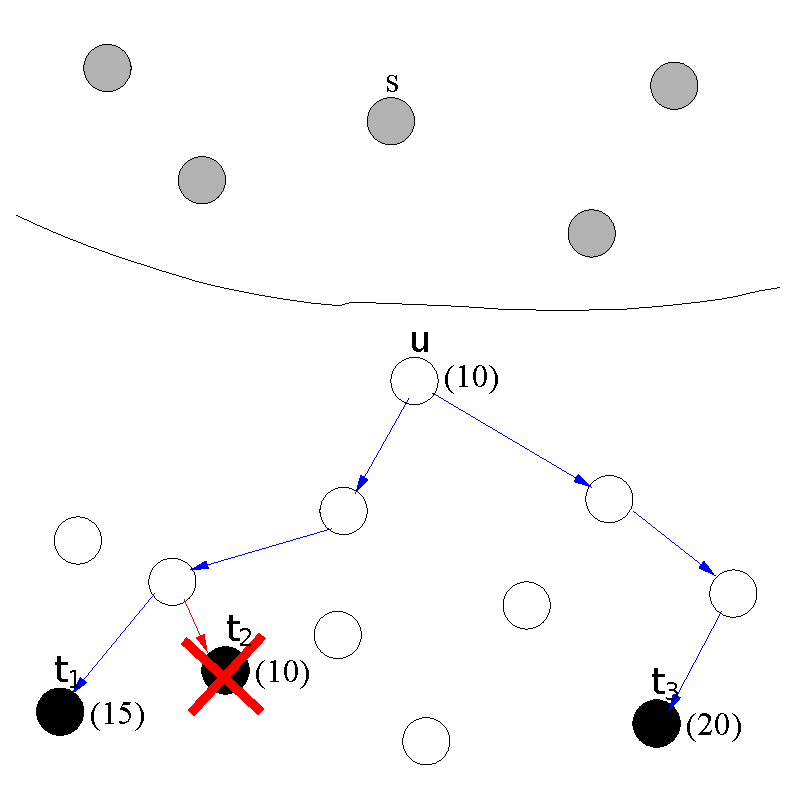
\includegraphics[scale=0.45]{imagens/neigh_color}
\label{fig:fig}
\end{figure}
\tiny
%\small
\begin{align*}
d(u,t_1,G(U)) &= 15 &d(s,u,G) + d(u,t_1,G(U)) &= 10 + 15 \leq 2 \cdot 15 \\
d(u,t_2,G(U)) &= 12 \Rightarrow &d(s,u,G) + d(u,t_1,G(U)) &= 10 + 12 > 2 \cdot 10 \Rightarrow \Delta-neigh(u) = \{t_1,t_3\} \\
d(u,t_3,G(U)) &= 25 &d(s,u,G) + d(u,t_1,G(U)) &= 10 + 25 \leq 2 \cdot 20
\end{align*}
\end{frame}

\begin{frame}{Cômputo da $\sqrt{l}$-partition (Fase 1)}
  \begin{itemize}
    \item A $\sqrt{l}$-partition divide $V$ em dois conjuntos disjuntos: $C$ e $U$.
    \item $\Delta$-neigh$(u)$ ($\forall u \in U$) deve conter no máximo $\sqrt{l}$ terminais.
    \item Partição computada através da eliminação dos \emph{$\sqrt{l}$-bad nodes}.
    \item Um nó $u$ é um $\sqrt{l}$-bad node se possui mais de $\sqrt{l}$ terminais em $\Delta$-neigh$(u)$.
  \end{itemize}
\end{frame}

\begin{frame}{Procedimento para cômputo da $\sqrt{l}$-partition (Fase 1)}
\begin{algorithm}[H]
\label{alg:compute_partition}
$C \gets \lbrace s \rbrace$, $U \gets V \setminus \lbrace s \rbrace$, $Roots \gets \emptyset$\\
\While{$G(U)$ contains a $\sqrt{l}$-bad node $v$}{
  Let $Cl(v)$ be the $\lfloor \sqrt{l} \rfloor$ uncovered terminals closest to $v$ in $G(U)$\\
  Let $T_v$ be a shortest path arborescence leading from $v$ to $Cl(v)$ in $G(U)$\\
  $C \gets C \cup V(T_v)$, $U \gets U \setminus V(T_v)$, $Roots \gets Roots \cup \lbrace v \rbrace$\\
}
Let $H(V_H,E_H)$ be the forest formed by the union of $T_v$, $\forall v \in Roots$\\
Output $(C,U,Roots, H)$
\caption{CompPar(G=(V, E), s, k)} 
\end{algorithm}
\end{frame}

\begin{frame}{CompPar - Grafo de entrada}
\begin{itemize}
  \item $t = 2$
\end{itemize}
\begin{figure}[H]
\centering
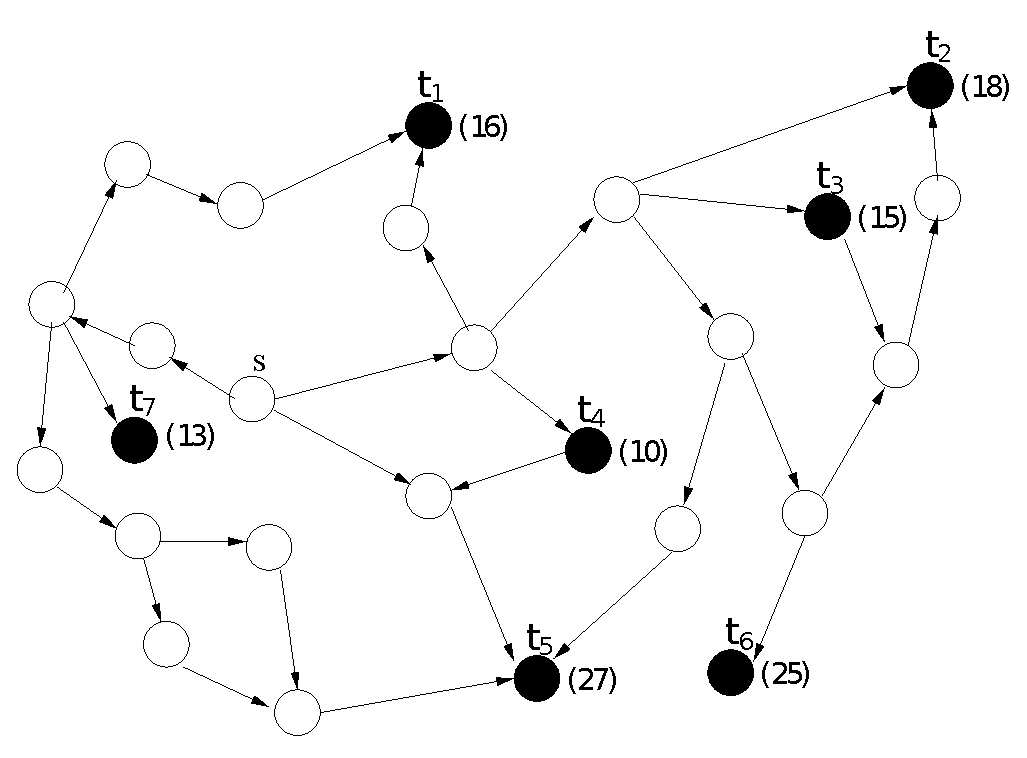
\includegraphics[scale=0.45]{imagens/compPar}
\label{fig:fig}
\end{figure}
\end{frame}

\begin{frame}{CompPar - $\sqrt{k}$-bad node}
\begin{itemize}
  \item $t = 2$
\end{itemize}
\begin{figure}[H]
\centering
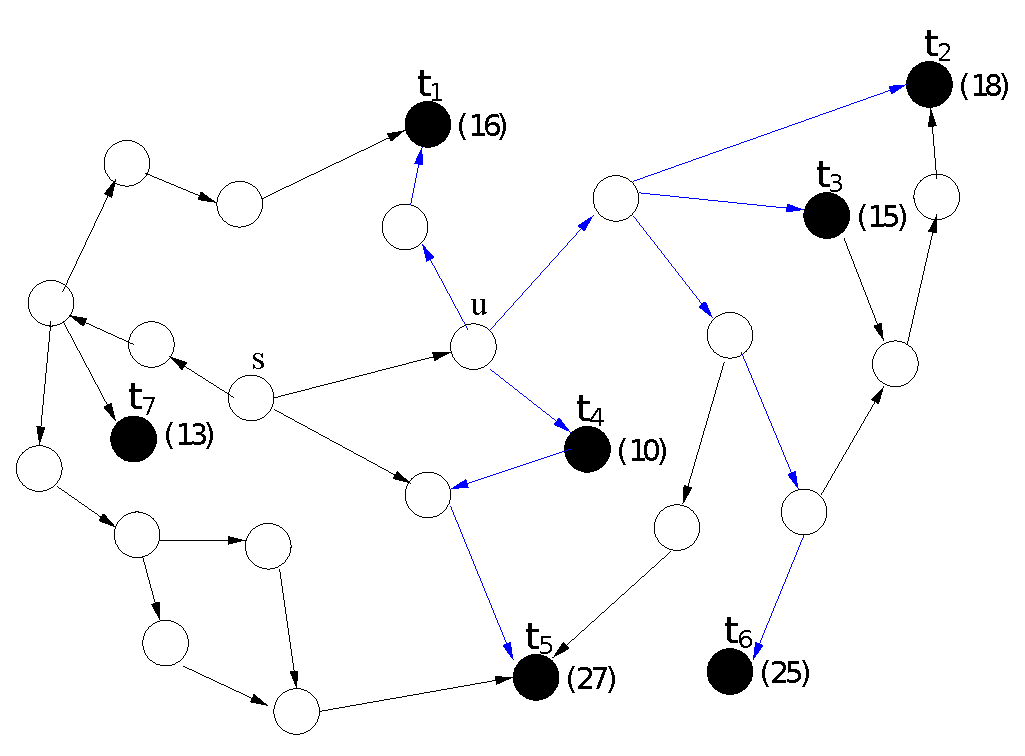
\includegraphics[scale=0.45]{imagens/compPar_bad1}
\label{fig:fig}
\end{figure}
%\small
\footnotesize
\begin{itemize}
  \item $u$ é $\sqrt{k}$-bad node.
  \item $d(s,u,G) = 5$; $d(u,t_4,G(u)) = 5$, $d(u,t_3,G(u)) = 10$, $d(u,t_1,G(u)) = 11$, $d(u,t_2,G(u)) = 13$, $d(u,t_6,G(u)) = 20$, $d(u,t_5,G(u)) = 22$.
\end{itemize}
\end{frame}

\begin{frame}{CompPar - $\lfloor \sqrt{l} \rfloor$ terminais mais próximos em $UT$}
\begin{itemize}
  \item $t = 2$
\end{itemize}
\begin{figure}[H]
\centering
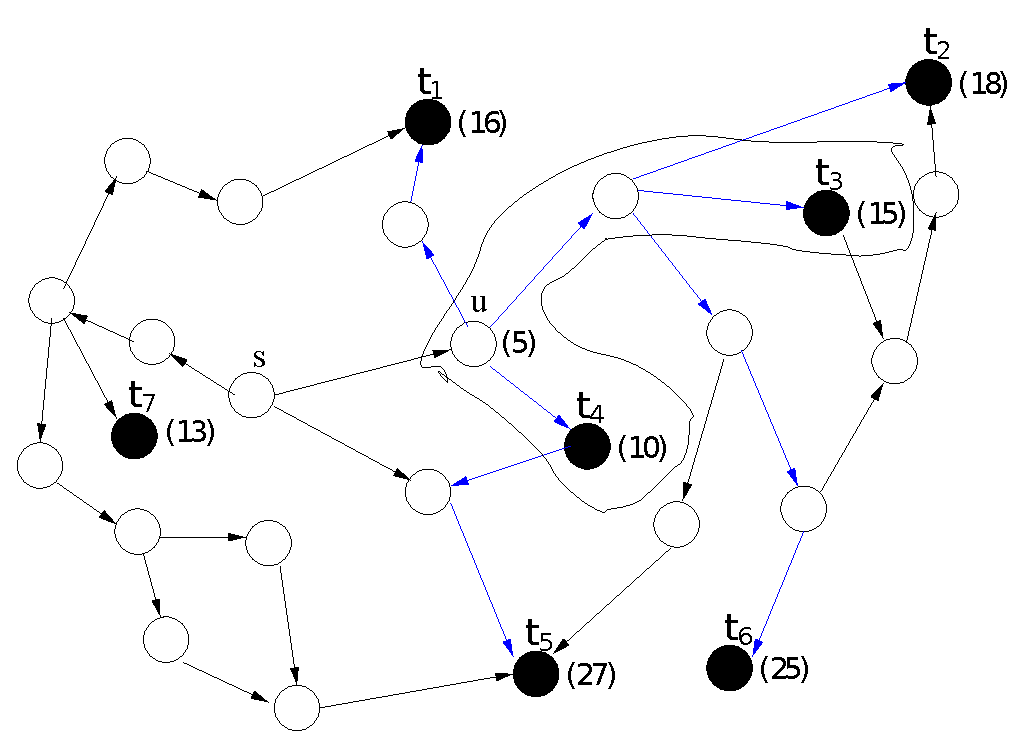
\includegraphics[scale=0.45]{imagens/compPar_tree1}
\label{fig:fig}
\end{figure}
%\small
%\footnotesize
%\begin{itemize}
%  \item $u$ é $\sqrt{k}$-bad node.
%  \item $d(s,u,G) = 5$; $d(u,t_4,G(u)) = 5$, $d(u,t_3,G(u)) = 10$, $d(u,t_1,G(u)) = 11$, $d(u,t_2,G(u)) = 13$, $d(u,t_6,G(u)) = 20$, $d(u,t_5,G(u)) = 22$.
%\end{itemize}
\end{frame}

\begin{frame}{CompPar - Eliminando os nós cobertos}
\begin{itemize}
  \item $t = 2$
\end{itemize}
\begin{figure}[H]
\centering
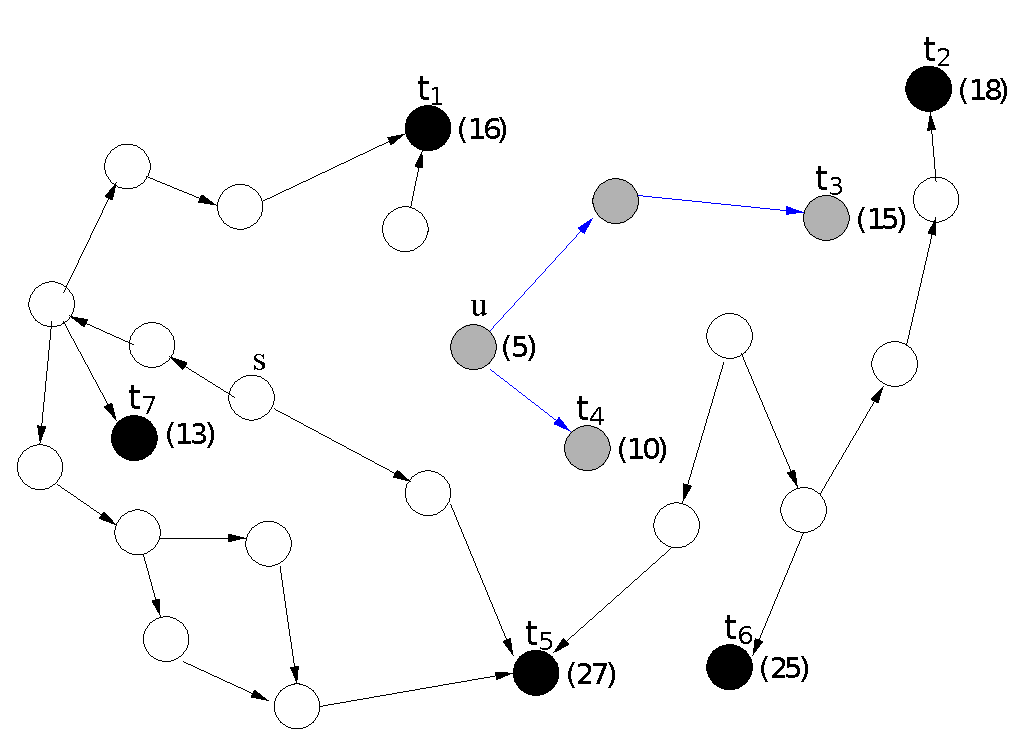
\includegraphics[scale=0.45]{imagens/compPar_cov1}
\label{fig:fig}
\end{figure}
%\small
%\footnotesize
\begin{itemize}
  \item $Root = \{u\}$.
\end{itemize}
\end{frame}

\begin{frame}{CompPar - $\sqrt{k}$-bad node}
\begin{itemize}
  \item $t = 2$
\end{itemize}
\begin{figure}[H]
\centering
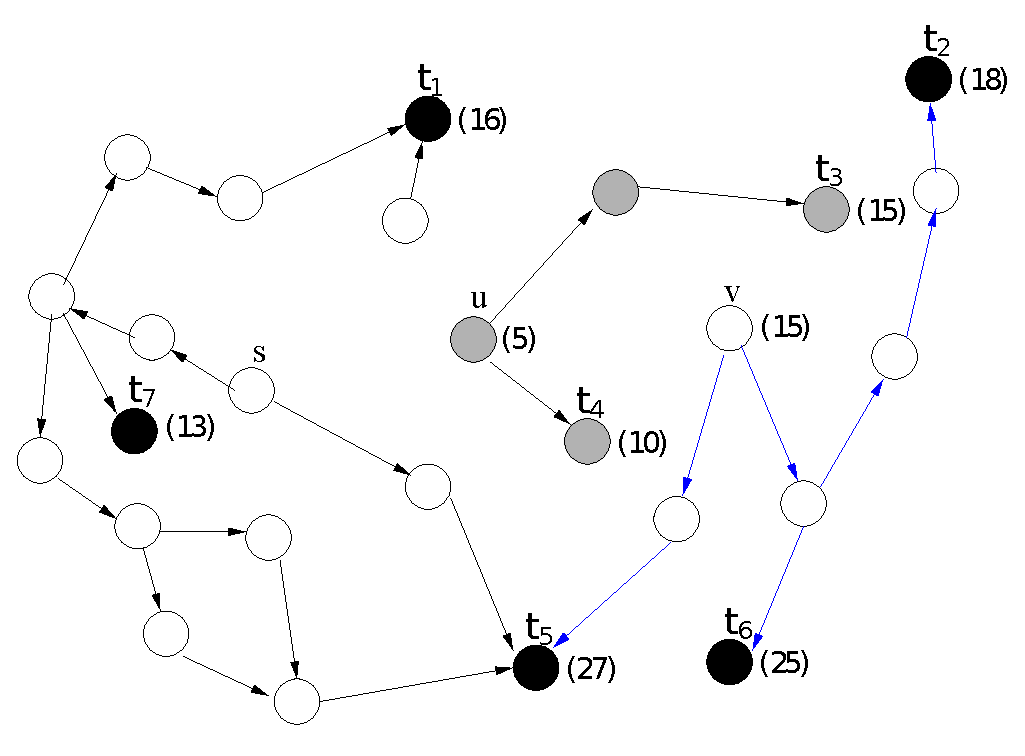
\includegraphics[scale=0.45]{imagens/compPar_bad2}
\label{fig:fig}
\end{figure}
%\small
\footnotesize
\begin{itemize}
  \item $v$ é $\sqrt{k}$-bad node.
  \item $d(v,t_6,G(u)) = 10$, $d(v,t_2,G(u)) = 20$, $d(v,t_5,G(u)) = 24$.
\end{itemize}
\end{frame}


\begin{frame}{CompPar - $\lfloor \sqrt{l} \rfloor$ terminais mais próximos em $UT$}
\begin{itemize}
  \item $t = 2$
\end{itemize}
\begin{figure}[H]
\centering
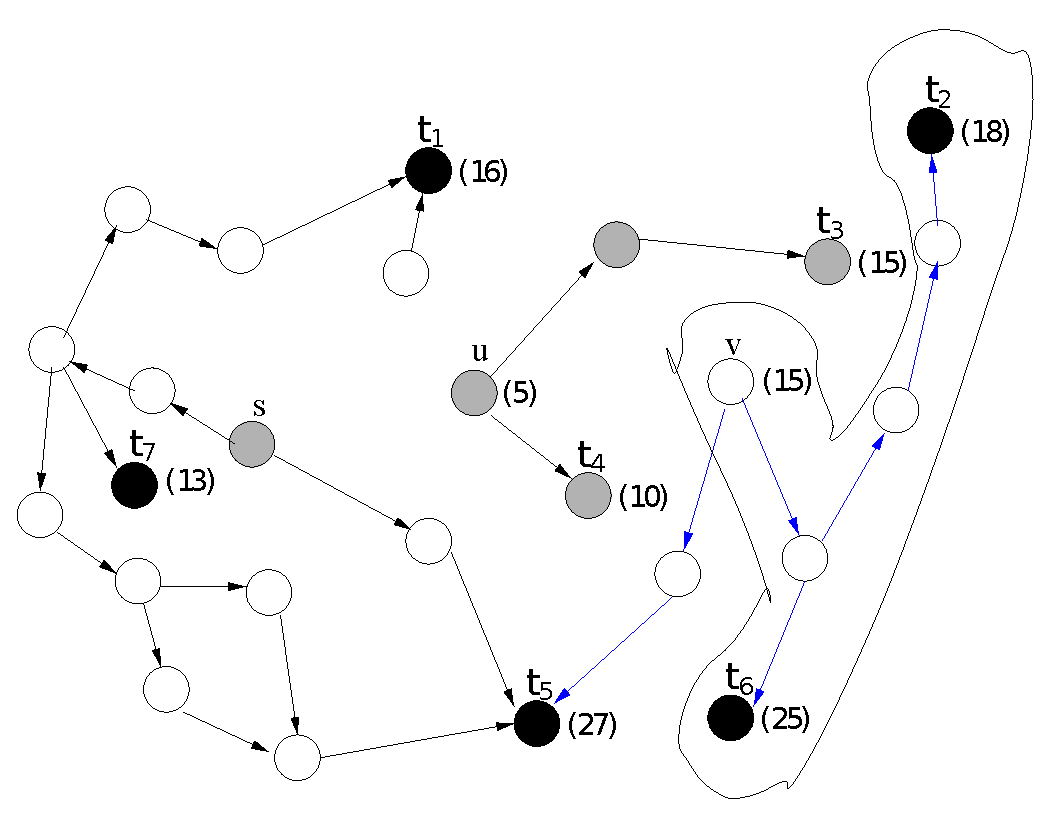
\includegraphics[scale=0.45]{imagens/compPar_tree2}
\label{fig:fig}
\end{figure}
%\small
%\footnotesize
%\begin{itemize}
%  \item $u$ é $\sqrt{k}$-bad node.
%  \item $d(s,u,G) = 5$; $d(u,t_4,G(u)) = 5$, $d(u,t_3,G(u)) = 10$, $d(u,t_1,G(u)) = 11$, $d(u,t_2,G(u)) = 13$, $d(u,t_6,G(u)) = 20$, $d(u,t_5,G(u)) = 22$.
%\end{itemize}
\end{frame}

\begin{frame}{CompPar - Eliminando os nós cobertos}
\begin{itemize}
  \item $t = 2$
\end{itemize}
\begin{figure}[H]
\centering
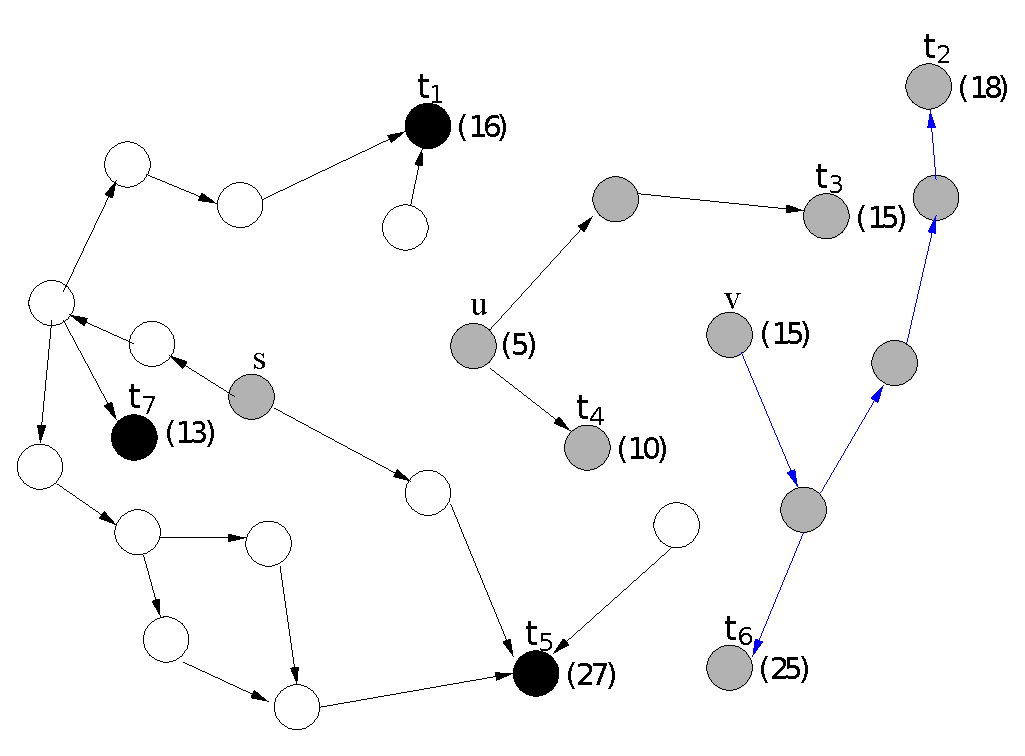
\includegraphics[scale=0.45]{imagens/compPar_cov2}
\label{fig:fig}
\end{figure}
%\small
%\footnotesize
\begin{itemize}
  \item $Root = \{u, v\}$.
\end{itemize}
\end{frame}

\begin{frame}{Algoritmo \ref{alg:compute_partition}: lemas}
\begin{lema} 
\label{lem:proc_comppar}
\cite{Elkin2006} O par $(C, U)$ gerado pelo Algoritmo \ref{alg:compute_partition} é uma $\sqrt l$-\emph{partition}.
\end{lema}

\begin{lema} 
\label{lem:roots_cardinality}
\cite{Elkin2006} $|Roots| \le \sqrt{l} + 2$.
%nao estou convencido deste valor
\end{lema}

\end{frame}

\begin{frame}{Construção de caminhos para $t \in CT$}
  \begin{itemize}
    \item Algoritmo \ref{alg:compute_graph_first_phase} descreve o procedimento para construção de um grafo que contém caminhos de $s$ para $t \in CT$ e que satisfaz $k \cdot dist(s,t,G)$.
  \end{itemize}

\begin{algorithm}[H]
%$Roots \gets \ref{alg:compute_partition}$\\
$A_{Roots} \gets SPT(s,Roots,G)$\\
%$H(V_H,E_H) \gets \varnothing$\\
%\ForEach{$u \in Roots$}{
%  $H \gets H \cup T_u$\\
%}
%Let $S_{leaves}$ be the set of leaves of all $T_u$, $\forall u \in Roots$\\
$G_{\sqrt{l}-Par} \gets A_{Roots} \cup H(V_H, E_H)$\\
$C \gets V(G_{\sqrt{l}-Par})$, $U \gets V \setminus C$\\
Output $(C,U,G_{\sqrt{l}-Par})$
\caption{CompGraphFirstPh(G, s, Roots, H)} 
\label{alg:compute_graph_first_phase}
\end{algorithm}

\begin{itemize}
  \item Terminais em $G_{\sqrt{l}-Par}$ respeitam a restrição de spanner.
\end{itemize}

\end{frame}

\begin{frame}{Limite no grau máximo de $G_{\sqrt{l}-Par}$ (Algoritmo \ref{alg:compute_graph_first_phase})}
  \begin{lema}
    \label{lem:roots_size}
    O grau máximo dos nós em $G_{\sqrt{l}-Par}$ é $\leq 2\sqrt{l} + 2$
  \end{lema}
\hypertarget{roots_size}{}
\hyperlink{roots_size_slide}{\beamergotobutton{Prova}}
\end{frame}

\begin{frame}{Problema do \emph{Multiple Set-Cover} (MSC)}
  \begin{itemize}
    \item Seja $\beta(V_1,V_2,E)$ um grafo bipartite. Um conjunto $S \subseteq V_1$ é denominado um \emph{set-cover} de $V_2$ se $N(S,\beta) = V_2$.
    \item Definição formal do MSC:
    \begin{itemize}
      \item Entrada: Um grafo bipartite $\beta(V_1,V_2,E)$ com $|V_1| + |V_2| = n$. $V_1 = \dot \bigcup_{j=1}^{d}A_j$.
      \item Saída: Um \emph{set-cover} $S \subset V_1$ de $V_2$ que minimiza $val(S)$, onde $val(S) = max\lbrace |S \cap A_i| \rbrace_{i=1}^{d}$.
    \end{itemize}
  \end{itemize}
\end{frame}

\begin{frame}{Exemplo do MSC}
\begin{figure}[H]
\centering
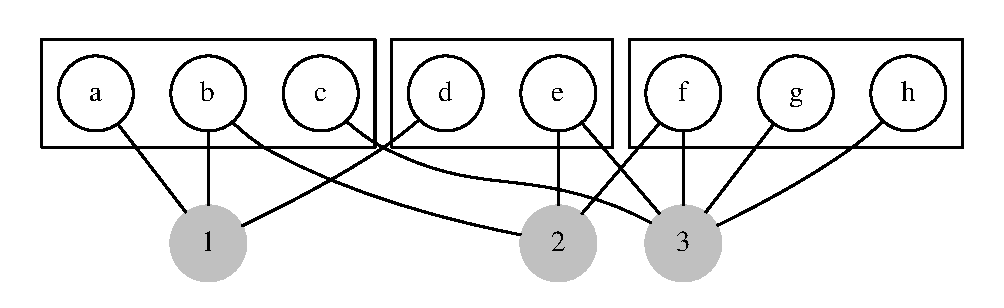
\includegraphics[scale=0.60]{imagens/msc}
\label{fig:msc}
\end{figure}

\begin{itemize}
  \item $V_1 = \lbrace a,b,c,d,e,f,g,h \rbrace$, $V_2 = \lbrace 1,2,3 \rbrace$.
  \item Os set-covers $S_1 = \lbrace a,e \rbrace$, $S_2 = \lbrace c,d,f \rbrace$ e $S_3 = \lbrace b,f \rbrace$ são soluções ótimas, pois $val(S_1) = val(S_2) = val(S_3) = 1$.
\end{itemize}
\end{frame}

\begin{frame}{Solução de aproximação para o MSC}
\begin{teorema}
  \label{teorema:fator_aproximacao}
  \cite{Chekuri2004}. Existe uma algoritmo guloso com fator de aproximação de $(\log |V_2| + 1)$ para o problema do MSC.
\end{teorema}
\end{frame}

\begin{frame}{Cobrindo nós em $UT$ através do MSC (Fase 2)}
\begin{itemize}
  \item Utilização de uma instância do MSC para constuir caminhos para os nós em $UT$ ao passo que o grau é limitado (similar a \cite{Elkin2006}).
  \item Fase dividida em duas partes: utilização do MSC para encontrar um subconjunto de nós cobertos; em sequência caminhos para os terminais em $UT$ a partir destes nós 
são definidos.
  \item Definição da instância $\beta=(V_1, V_2, \varepsilon)$ do MSC:
  \begin{itemize}
    \item $V_1$ é formado por \emph{pseudo nós}. $V_1 = \lbrace x_{u,v} : u \in C, v \in U, (u,v) \in E \rbrace$.
    \item $V_2 = UT$.
    \item Existe uma aresta em $\varepsilon$ entre $x_{u,v}$ e $t \in V_2$ sse $dist(s, u, G) + C(u, v) + dist(v,t,G(U)) \leq k \cdot dist(s,t,G)$.
    \item Seja $A_u = \lbrace x_{u,v} :  v \in N(u, G(U)) \rbrace$. $V_1 = \dot \bigcup_{u \in C}A_u$.
  \end{itemize}
\end{itemize}
\end{frame}

\begin{frame}{Instância do MSC}
\scriptsize  
\begin{itemize}
  \item $t = 2$
  \item Caminhos coloridos satisfazem a relação $dist(s, u, G) + C(u, v) + dist(v,t,G(U)) \leq k \cdot dist(s,t,G)$.
\end{itemize}
\begin{figure}[H]
\centering
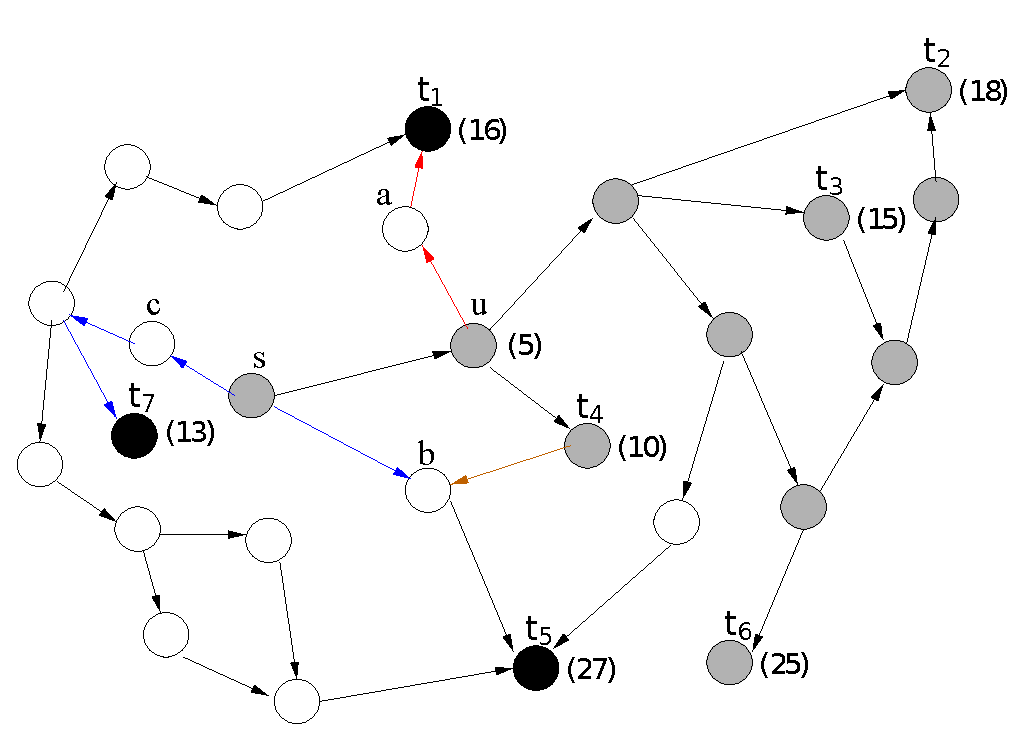
\includegraphics[scale=0.45]{imagens/mscInstance}
\label{fig:fig}
\end{figure}

\scriptsize
\begin{itemize}
  \item <2-> $V_1 = \{ X_{u,a}, X_{t_4,b}, X_{s,b}, X_{s,c} \}$, partição de $V_1 = \{ \{ X_{u,a} \}, \{ X_{t_4,b} \}, \{ X_{s,b}, X_{s,c} \} \}$.
  \item <2-> $V_2 = \{ t_1, t_5, t_7 \}$.
  \item <2-> $\varepsilon = \{ (X_{u,a}, t_1), (X_{t_4,b}, t_5), (X_{s,b}, t_5), (X_{s,c}, t_7) \}$.
\end{itemize}

\end{frame}

\begin{frame}{Limite superior para a solução da instância do MSC}
  \begin{lema}
    \label{lem:val_solution}
    A instância $\beta=(V_1, V_2, \varepsilon)$ do MSC admite uma solução $S^* \subseteq V_1$ t.q. $val(S^*) \leq d^*$.
  \end{lema}
\hypertarget{val_solution}{}
\hyperlink{val_solution_slide}{\beamergotobutton{Prova}}
\end{frame}

\begin{frame}{Limite da interseção entre a solução do MSC e cada partição de $V_1$}
  \begin{lema}
    \label{lem:max_pseudo_node_degree}
    Seja $D$ uma solução para $\beta=(V_1, V_2, \varepsilon)$ com $V_1 = \dot \bigcup_{v \in C}A_v$ usando o algoritmo apresentado em \cite{Chekuri2004}. 
Então $max_{v \in C}|D \cap A_v| = O(\log l)\cdot d^*$.
  \end{lema}
\hypertarget{max_pseudo_node_degree}{}
\hyperlink{max_pseudo_node_degree_slide}{\beamergotobutton{Prova}}
\end{frame}

\begin{frame}{Algoritmo de Aproximação}
\begin{algorithm}[H]
Input: $G=(V, E)$, $s \in V$, $T \subset V$, $k$ \linebreak
Output: $\mathcal{A}_f =(V_{\mathcal{A}_f}, E_{\mathcal{A}_f})$ \linebreak
\BlankLine
  $(C, U, Roots, H) \gets$ \emph{CompPar}($G, s, k$) \\ 
  $(C, U, G_{\sqrt{l}-Par})\gets $\emph{CompGraphFirstPh}$(G,s,Roots,H)$ \\	
  Build the MSC instance $\beta = (V_1, V_2, \varepsilon)$ \\
  $D \gets $ Apply approximation algorithm \cite{Chekuri2004} on $\beta$\\
  $\varGamma(V_{\varGamma},E_{\varGamma}), V_{\varGamma} \gets \emptyset, E_{\varGamma} \gets \emptyset$\\
  \ForEach{$t \in V_2$}{
    Choose $x_{u, v} \in D$ : $(x_{u, v}, t) \in \varepsilon$ and \hspace*{1.5cm} $C(u, v) + dist(v,t,G(U))$ is minimum \\
    $s \gets sp(v, t, G(U))$ \\
    $V_{\varGamma} \gets V_{\varGamma} \cup \{u\} \cup V(s)$ \\ %, \forall q, q \in S_{ter}$\\% \wedge q \notin V_{\varGamma}$ \\
    $E_{\varGamma} \gets E_{\varGamma} \cup \{(u, v)\} \cup E(s)$ \\ %, \forall q, q \in S_{ter}$\\% \wedge q \notin V_{\varGamma}$ \\
 }
  $G_f \gets G_{\sqrt{l}-Par} \cup \varGamma(V_\varGamma,E_\varGamma)$ \\
  $\mathcal{A}_f \gets SPT(s, T, G_f)$
\caption{Algoritmo de Aproximação para o DSMDStP} 
\label{alg:approximation}
\end{algorithm}
\end{frame}

\begin{frame}{Grau máximo de $G_f$}
  \begin{lema}
    \label{lem:max_degree}
    O grau máximo dos nós em $G_f$ é $\leq 2\sqrt{l} + 2 + O(\log l) \cdot d^*$.
  \end{lema}
\hypertarget{max_degree}{}
\hyperlink{max_degree_slide}{\beamergotobutton{Prova}}
\end{frame}

\begin{frame}{Custo máximo dos caminhos para os terminais}
  \begin{lema}
    \label{lem:cost_guaranteed}
$\forall t \in T$, $dist(s,t,G_f) \leq k \cdot ( dist(s,t,G) + dist(s,t_{max},G))$, 
where $t_{max} \in \{t' | 
(t' \in T) \land (\forall t'' \in T : dist(s,t'',G) \le dist(s,t',G))\}$.
  \end{lema}
\hypertarget{cost_guaranteed}{}
\hyperlink{cost_guaranteed_slide}{\beamergotobutton{Prova}}
\end{frame}

\begin{frame}{Teorema Principal}
  \begin{teorema}
    \label{teorema:final_theorem}
    Algoritmo \ref{alg:approximation} gera uma arborescência $\mathcal{A}_f$ com grau máximo $2\sqrt{k} + 2 + O(\log l) \cdot d^*$ e que possui caminhos entre $s$ e 
cada terminal $t \in T$ com custo $\le k \cdot ( dist(s,t,G) + dist(s,t_{max},G))$.
  \end{teorema}
\hypertarget{final_theorem}{}
\hyperlink{final_theorem_slide}{\beamergotobutton{Prova}}
\end{frame}

\begin{frame}{Complexidade}
\label{comp:comp_approx}
\begin{itemize}
  \item $O((\log{|T|})(|V|^3|T|^2)$.
\end{itemize}
\hypertarget{comp_approx}{}
\hyperlink{comp_approx_slide}{\beamergotobutton{Detalhe}}
\end{frame}

\subsection{SIM}

\begin{frame}{Resumo da heurística}
  \begin{itemize}
    \item SIM: acrônimo para \emph{Sliced and Iterative Msc}.
    \begin{itemize}
      \item Aplicação iterativa do algoritmo para o MSC.
      \item O conjunto de terminais é 'fatiado' e o MSC é aplicado é um conjunto menor se comparado ao algoritmo de aproximação.
    \end{itemize}
    \item Em cada iteração, os próximos $\lfloor\sqrt{l}\rfloor$ terminais (não cobertos) são cobertos $\rightarrow Next^{\sqrt{l}}_{ter}$.
    %\item Apenas nós que não fizeram parte de uma solução para uma prévia execução do MSC são considerados na próxima instância do MSC.
    %\begin{itemize}
    %  \item Se necessário, nós que já fizeram parte de uma solução também serão considerados.
    %\end{itemize}
  \end{itemize}
\end{frame}

\begin{frame}{SIM}
\scalebox{0.66}{
\begin{algorithm}[H]
Input: $G=(V, E)$, $s \in V$, $T \subset V$, $k$\linebreak
Output: $\mathcal{A}_f=(V_{\mathcal{A}_f}, E_{\mathcal{A}_f})$\linebreak
\BlankLine
  $C \gets \{s\}$, $U \gets V \setminus \lbrace s \rbrace$, $Marked \gets \emptyset$, $l \gets |T|$ \\
  \While{$UT \neq \emptyset$}{
    Set $V_1, V_2$ and $\varepsilon$ using the current values of $C$, $U$, $Marked$ and $Next^{\sqrt{l}}_{ter}$ \\
    \ForEach{$t : t \in V_2$ and $\nexists$ edge $(x,t) \in \varepsilon$ for any $x$}{
      Let $x_{u, v}$ be a pseudo node such that: \linebreak
	\hspace*{0.4cm} $u \in Marked$, \linebreak
	\hspace*{0.4cm} $u$ has the smallest out-degree and 
	\hspace*{0.4cm} $C(u,v) + dist(v,t,G(U)) \leq k \cdot dist(s,t,G)$\\
      $V_1$ $\gets$ $V_1 \cup \{x_{u,v}\}$,  $\varepsilon \gets \varepsilon \cup \{(x_{u,v},t)\}$ \\
    }
    $D \gets $ Apply approximation algorithm \cite{Chekuri2004} on \hspace*{0.7cm} $\beta(V_1, V_2, \varepsilon)$\\
    $\varGamma(V_{\varGamma},E_{\varGamma}) \gets \emptyset$\\
  \ForEach{$t \in V_2$}{
    Choose a node $x_{u, v} \in D: (x_{u, v},t) \in \varepsilon$ and \linebreak
	\hspace*{0.5cm} $C(u, v) + dist(v,t,G(U))$ is minimum\\
    $Marked \gets Marked$ $\cup$ $\{u\}$ \{for which $x_{(u,v)}$ \linebreak
	\hspace*{0.5cm} was chosen in the last line\} \\
    $s \gets sp(v, t, G(U))$ \\
    $V_{\varGamma} \gets V_{\varGamma} \cup \{u\} \cup V(s)$ \\ 
    $E_{\varGamma} \gets E_{\varGamma} \cup \{(u, v)\} \cup E(s)$ \\ 
  }
    $C \gets C \cup V_\varGamma$, $U \gets U \setminus V_\Gamma$\\
    $\mathcal{A}_f \gets \mathcal{A}_f \cup \Gamma(V_\Gamma,E_\Gamma)$
  }
\caption{SIM - Sliced and Iterative MSC} 
\label{alg:sim}
\end{algorithm}  
}
\end{frame}

\begin{frame}{Existência de um caminho para todo terminal em $\mathcal{A}_f$}
  \begin{lema}
    \label{lem:terminals_covered}
    Seja $\mathcal{A}_f$ a arborescência gerada por SIM. $\forall t \in T$, existe um caminho entre $s$ e $t$ em $\mathcal{A}_f$.
  \end{lema}
\hypertarget{terminals_covered}{}
\hyperlink{terminals_covered_slide}{\beamergotobutton{Prova}}
\end{frame}

\begin{frame}{Número de iterações do SIM}
  \begin{lema}
    \label{lem:number_iterations}
    O número de iterações do SIM é limitado por $\lfloor\sqrt{l}\rfloor + 2$.
  \end{lema}
\hypertarget{number_iterations}{}
\hyperlink{number_iterations_slide}{\beamergotobutton{Prova}}
\end{frame}

\begin{frame}{Grafo gerado por SIM é uma arborescência}
  \begin{lema}
    \label{lem:sim_output_arborescence}
    Seja $\mathcal{A}_f$ o grafo gerado por SIM. $\mathcal{A}_f$ é uma arborescência.
  \end{lema}
\hypertarget{sim_output_arborescence}{}
\hyperlink{sim_output_arborescence_slide}{\beamergotobutton{Prova}}
%\end{frame}
%\begin{frame}{Grafo gerado por SIM é uma arborescência}
\end{frame}

\begin{frame}{Custo máximo dos caminhos gerados por SIM}
  \begin{teorema}
    \label{teo:cost}
    Seja $\mathcal{A}_f$ a arborescência gerada por SIM. $\forall t \in T, dist(s,t,\mathcal{A}_f) \leq (\lfloor\sqrt{l}\rfloor+2) \cdot k \cdot dist(s,t,G)$.
  \end{teorema}
\hypertarget{cost}{}
\hyperlink{cost_slide}{\beamergotobutton{Prova}}
\end{frame}

\begin{frame}{Complexidade}
\begin{itemize}
  \item $O((\log \sqrt{|T|})(|V|^3|T| \sqrt{|T|}))$.
\end{itemize}
\hypertarget{comp_sim}{}
\hyperlink{comp_sim_slide}{\beamergotobutton{Detalhe}}
\end{frame}

\section{Experimentos}
\begin{frame}{Parâmetros e detalhes da implementação}
  \begin{itemize}
    \item Algoritmos implementados em Java.
    \item Nós espalhados em uma área de $500 x 500$ no espaço Euclideano.
    \item Alcance de cada nó é de 125 unidades de medida.
    \item Faixas de valores:
    \begin{itemize}
      \item Rede: 60 .. 300.
      \item Terminais: 10 .. 50.
      \item Fator de dilatação: 1 .. 2.
    \end{itemize}
    \item 30 simulações para cada cenário.
  \end{itemize}
\end{frame}

\begin{frame}{Algoritmos e Métricas}
\begin{itemize}
  \item <2-> Algoritmos:
  \begin{itemize}
    \item DSMDStP é um problema novo.
    \item Comparamos com o SPT.
    \begin{itemize}
      \item Satisfaz as restrições do problema.
      \item Algoritmo simples e eficiente*.
      \item Similaridades com os algoritmos propostos (principalmente APPROX).
    \end{itemize}
  \end{itemize}
  \item <3-> 4 métricas:
  \begin{itemize}
    \item <4-> Grau máximo.
    \item <5-> Razão de violação do custo (CVR): $\frac{\sum_{\forall t \in T_{vio}}\frac{dist(s,t,\mathcal{A}_f)}{k \cdot dist(s,t,G)}}{|T_{vio}|}$.
    \begin{itemize}
      \item Pior caso da razão de violação ($MAX\_CVR$).
    \end{itemize}
    \item <6-> Percentagem de terminais que violam restrições (PVT): $\frac{|T_{vio}|}{|T|} \cdot 100 \%$.
    \item <7-> Percentagem de cenários violados (PVR).
  \end{itemize}
\end{itemize}
\end{frame}

\begin{frame}{Grau x Rede}
\begin{figure}[H]
\centering
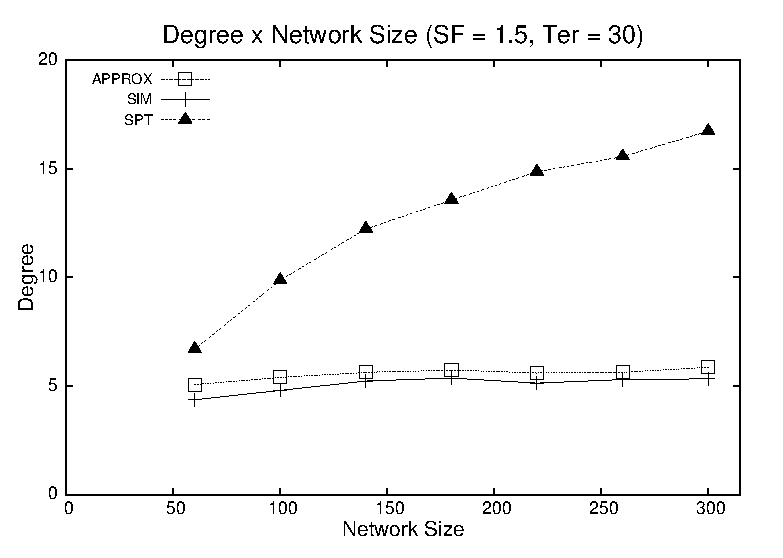
\includegraphics[scale=0.60]{imagens/defesa-grau_rede}
\label{fig:grau_rede}
\end{figure}
\begin{itemize}
  \item APPROX e SIM escalam bem.
  \item SPT possui grau 3x maior do que os outros algoritmos em redes densas.
\end{itemize}
\end{frame}

\begin{frame}{Grau x Terminais}
\begin{figure}[H]
\centering
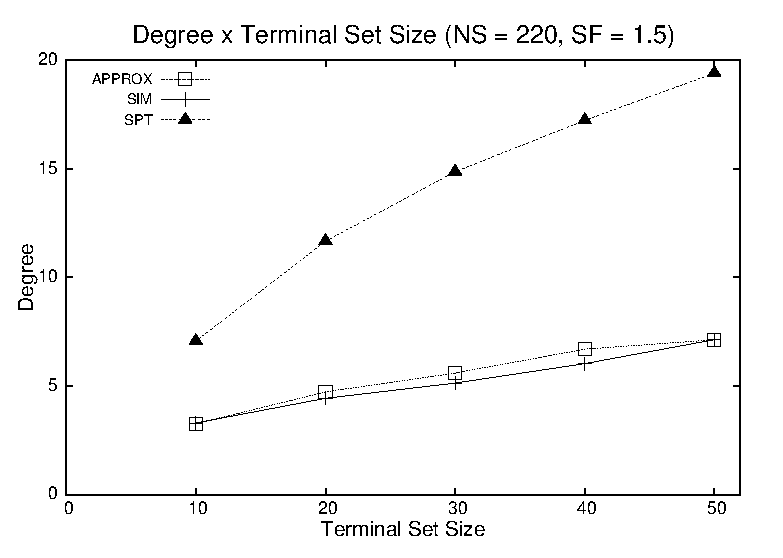
\includegraphics[scale=0.60]{imagens/defesa-grau_terminal}
\label{fig:grau_terminal}
\end{figure}
\begin{itemize}
  \item Crescrimento do grau para APPROX e SIM já era esperado.
  \begin{itemize}
    \item Em cada fase, o grau máximo do(s) algoritmo(s) é afetado pela quantidade de terminais.
  \end{itemize}
  \item Taxa de crescimento bem maior para SPT.
\end{itemize}
\end{frame}

\begin{frame}{Grau x Fator de Dilatação}
\begin{figure}[H]
\centering
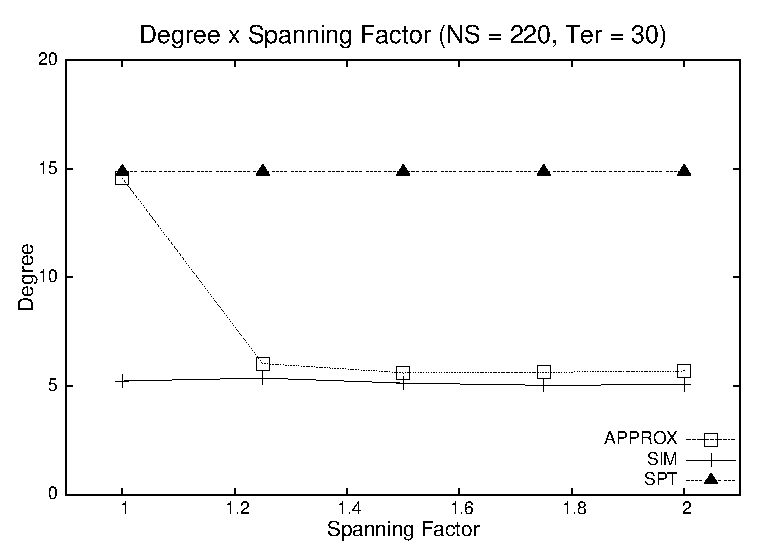
\includegraphics[scale=0.60]{imagens/defesa-grau_sf}
\label{fig:grau_sf}
\end{figure}
\begin{itemize}
  \item Comportamento de SIM é estável.
  \item APPROX escala bem, exceto para o caso restritivo do fator de dilatação.
  %\begin{itemize}
  %  \item Assemelha-se ao SPT pois os caminhos disponíveis para configurar a instância do MSC são os mesmos caminhos da árvore do SPT*.
  %\end{itemize}
\end{itemize}
\end{frame}

\begin{frame}{Grau x Rede, SF = 1}
\begin{figure}[H]
\centering
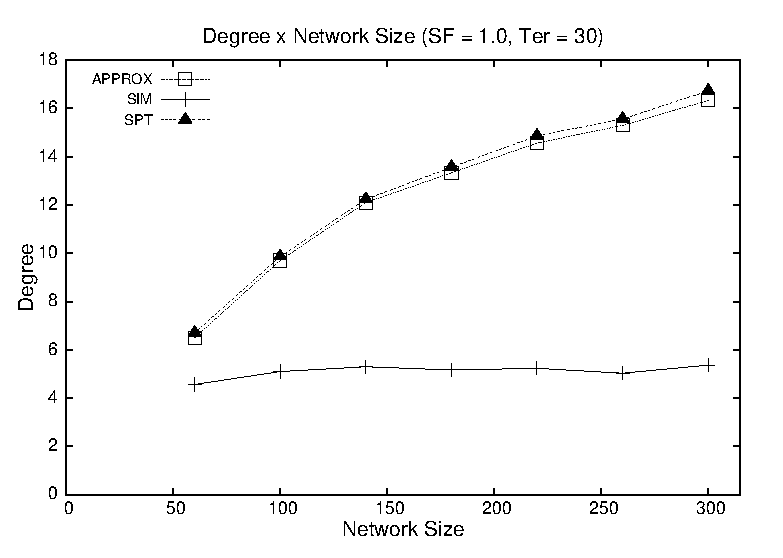
\includegraphics[scale=0.60]{imagens/defesa-grau_rede_sf1}
\label{fig:grau_rede_sf1}
\end{figure}
\begin{itemize}
  %\item Objetivo é manter os caminhos de custo mínimo.
  \item Curva do APPROX assemelha-se à curva do SPT.
  \begin{itemize}
    \item $<$ sf $\Leftrightarrow$ menos opções de caminhos para os terminais não-cobertos.
    \item Basicamente os caminhos que sobram fazem parte da árvore de custo mínimo (SPT).
  \end{itemize}
\end{itemize}
\end{frame}

\begin{frame}{CVR x Rede}
\begin{figure}[H]
\centering
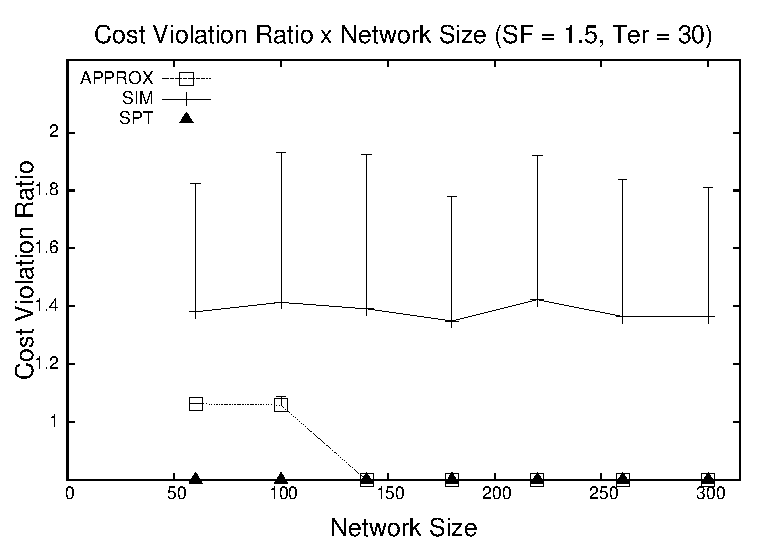
\includegraphics[scale=0.60]{imagens/defesa-cvr_rede}
\label{fig:cvr_rede}
\end{figure}
\begin{itemize}
  \item Valores de APROX próximos de 1, ou não há violação.
  \item SIM apresenta valores uniformes e baixos.
  \item MAX\_CVR abaixo de 2 para o SIM e próximo do CVR para APPROX.
\end{itemize}
\end{frame}

\begin{frame}{CVR x Terminais}
\begin{figure}[H]
\centering
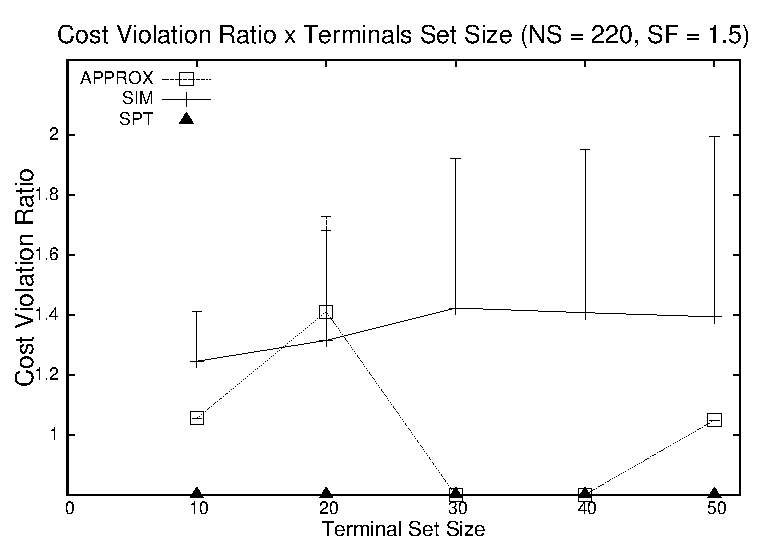
\includegraphics[scale=0.60]{imagens/defesa-cvr_terminal}
\label{fig:cvr_terminal}
\end{figure}
\begin{itemize}
  \item Comportamente semelhante ao gráfico anterior.
\end{itemize}
\end{frame}

\begin{frame}{CVR x Fator de dilatação}
\begin{figure}[H]
\centering
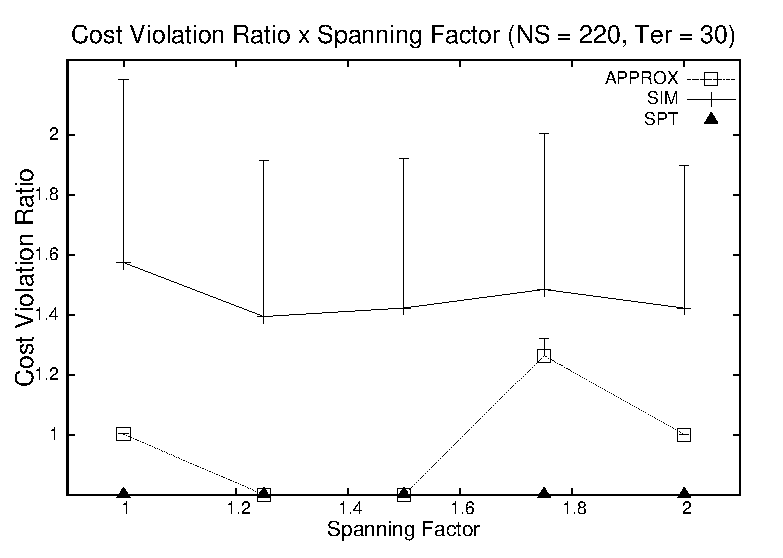
\includegraphics[scale=0.60]{imagens/defesa-cvr_sf}
\label{fig:cvr_sf}
\end{figure}
\begin{itemize}
  \item Comportamente semelhante ao gráfico anterior.
\end{itemize}
\end{frame}

\begin{frame}{PVT}
\begin{figure}[H]
\centering
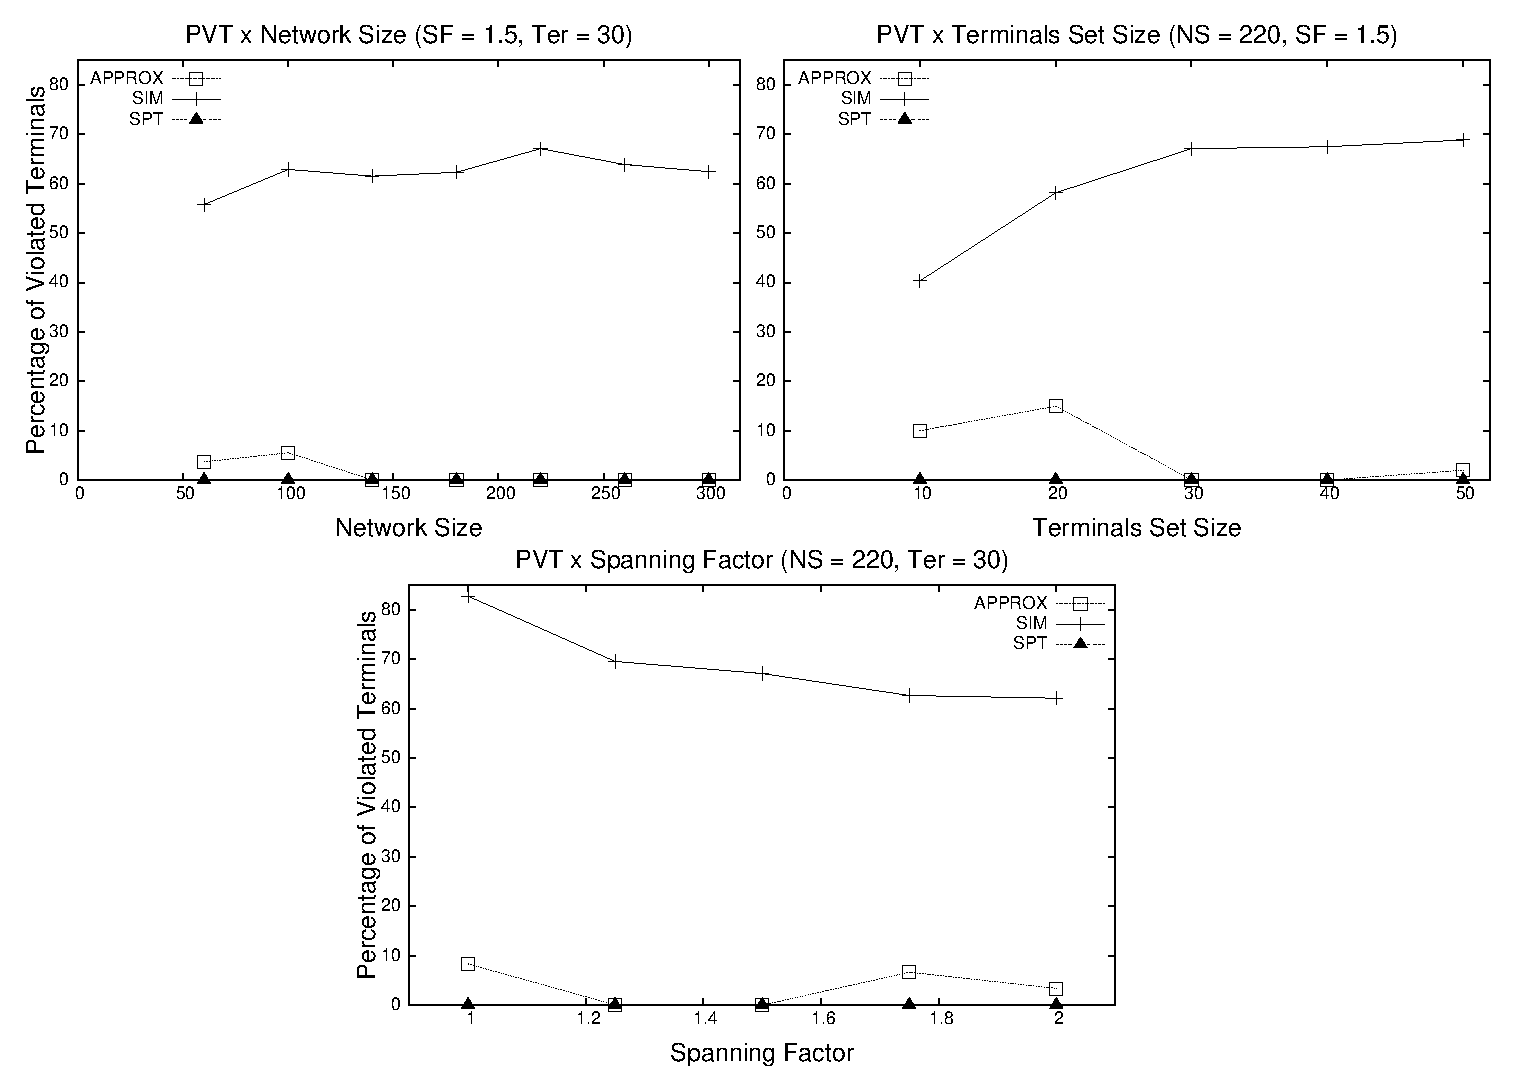
\includegraphics[scale=0.30]{imagens/violatedNodesRatio-220-3_graficos_nao_alinhados}
\label{fig:pvt_3}
\end{figure}
\begin{itemize}
  \item Percentagem pequena dos terminais que violam para o APPROX (10\%).
\end{itemize}
\end{frame}

\begin{frame}{PVR x Rede}
\begin{figure}[H]
\centering
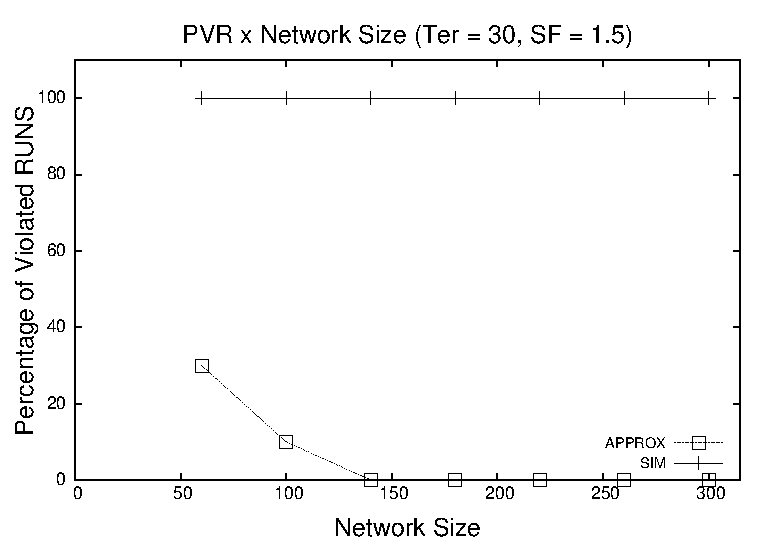
\includegraphics[scale=0.60]{imagens/defesa-pvr_rede}
\label{fig:pvr_rede}
\end{figure}
\begin{itemize}
  \item APPROX causa violação em uma percentagem relativamente baixa de cenários.
  \begin{itemize}
    \item Apenas um terminal é suficiente para considerar que ocorreu violação no cenário.
  \end{itemize}
\end{itemize}
\end{frame}

\begin{frame}{Experimentos - Resultado}
\begin{itemize}
  \item <1-> Grau baixo para os algoritmos propostos.
  \begin{itemize}
    \item <2-> Exceto para APPROX no pior cenário com relação ao FD.
    \item <2-> Neste cenário, APPROX equivale ao SPT com relação ao grau.
  \end{itemize}
  \item <3-> SIM possui melhor grau e escala bem.
  \item <4-> APPROX é melhor que SIM nas métricas que concerne a propriedade de spanner.
  \item <5-> Com APPROX, em metade das situações não ocorreu violação; na outra metade, a violação foi por um fator (CVR) baixo.
  \item <6-> Com relação ao spanner, SIM apresenta bons resultados para a principal métrica (CVR), a métrica qualitativa.
  \begin{itemize}
    \item <6-> CVR: 1.4.
    \item <6-> MAX\_CVR: 2.
  \end{itemize}
\end{itemize}
\end{frame}

\section{Função Submodular e Matroids}

\begin{frame}{Funções submodulares e Matroids}
\begin{itemize}
  \item MCG pode ser modelado através dos conceitos de \emph{funções submodulares} e \emph{matroids} (\cite{Calinescu2011}).
\end{itemize}
\hypertarget{matroid}{}
\hyperlink{matroid_slide}{\beamergotobutton{Formalismo}}
\end{frame}

\begin{frame}{Maximização de função submodular}
\begin{itemize}
  \item <1-> O problema abordado em \cite{Calinescu2011} foi o da maximização de função submodular sob restrição de uma matroid (SUB-M).
  \item <2-> Este problema já tinha sido abordado em outros trabalhos \cite{Nemhauser1978,Fisher1978}.
  \item <3-> Os autores em \cite{Calinescu2011} conseguem generalizar o resultado para qualquer tipo de matroid (incluindo matroid de partição), mantendo a garantia de 
aproximação ($(e/(e-1))$).
  \begin{itemize}
    \item <4-> O resultado dos autores é probabilístico:
    \begin{itemize}
      \item <5-> Garantia do grau passaria a ser probabilística.
      \item <6-> Para o MSC, o limite no número de iterações para cobrir todos os terminais seria probabilístico.
    \end{itemize}
  \end{itemize}
\end{itemize}
\end{frame}

\section{Conclusão}
\begin{frame}[allowframebreaks]{Conclusão}
\begin{itemize}
  \item Propomos um novo problema, denominado \emph{Árvore Steiner com Grau Mínimo e fator de dilatação k em Grafos Direcionados} (DSMDStP).
  \item Provamos que este problema não é aproximável sublogaritimicamente.
  \item Propomos duas soluções: um algoritmo de aproximação e uma heurística.
  \item Provamos as propriedades e garantias de ambos os algoritmos.
  \item Algoritmo de aproximação:
  \begin{itemize}
    \item Garantia do grau: $2\sqrt{|T|} + 2 + O(\log{|T|})\cdot d^*$.
    \item Custo máximo: $\le k \cdot ( dist(s,t,G) + dist(s,t_{max},G))$.
  \end{itemize}
  \item SIM:
  \begin{itemize}
    \item Custo máximo: $(|T| + 2) \cdot k \cdot dist(s,t,G)$.
  \end{itemize}
  \item Extensa simulação foi apresentada.
  \begin{itemize}
    \item Ambos os algoritmos apresentam grau muito baixo.
    \item SIM possui grau uniforme e apresentou melhores resultados que APPROX e SPT.
    \item A qualidade da violação apresentada é baixa (1.4 na média).
    \item APPROX apresentou resultados muito bons para a propriedade spanner:
    \begin{itemize}
      \item Em metade das situações não ocorreu violação.
      \item Na outra metade, a violação muito baixa qualitativamente (em média $1$ - praticamente sem violação) e quantitativamente.
    \end{itemize}
  \end{itemize}
\end{itemize}
\end{frame}

\begin{frame}{Trabalhos Futuros}
\begin{itemize}
  \item <2-> Tentar garantir as restrições de spanner.
  \item <3-> Solução distribuída.
  \item <4-> Modelar a solução através de função submodular e matroids.
\end{itemize}

\end{frame}


\begin{frame}{Definições preliminares}
\hypertarget{DTIME_slide}{}
  \begin{itemize}
    \item Algoritmo de aproximação por um fator $\alpha$ \cite{Williamson2011}: consistem em um algoritmo polinomial tal que para todas as instâncias do problema de otimização, 
produz uma solução cujo valor se aproxima do valor ótimo por um fator $\alpha$.
    \item Classe de complexidade \emph{DTIME} \cite{Arora2009}: Seja $T : \mathbb{R} \rightarrow \mathbb{R}$ uma função. Uma linguagem $L \in$  \textbf{DTIME}($T(n)$) sse 
existe uma máquina de Turing que decide $L$ em um tempo de execução de $c \cdot T(n)$, para uma constante $c > 0$. \hyperlink{DTIME}{\beamergotobutton{Back}}
  \end{itemize}
\end{frame}

\begin{frame}{Funções submodulares e Matroids \hyperlink{matroid}{\beamergotobutton{Voltar}}}
\hypertarget{matroid_slide}{}
\begin{itemize}
  %\item MCG pode ser modelado através dos conceitos de \emph{funções submodulares} e \emph{matroids} (\cite{Calinescu2011}).
  \item $f: 2^{X} \rightarrow \mathbb{R}^+$ é submodular sse $f(A \cup B) + f(A \cap B) \le f(A) + f(B)$.
  \item Matroid:
  \begin{itemize}
    \item Conjunto base $X$.
    \item Família de elementos independentes $I \subseteq 2^{X}$.
    \item Matroid é um par $M = (X,I)$ tal que:
    \begin{itemize}
      \item $\forall B \in I, A \subset B \Rightarrow A \in I$.
      \item $\forall A,B \in I; |A| < |B| \Rightarrow \exists x \in B \setminus A; A \cup x \in I$.
    \end{itemize}
  \end{itemize}
\end{itemize}
\end{frame}

\begin{frame}{Impossibilidade de aproximação sublogarítmica \hyperlink{not_approximable}{\beamergotobutton{Voltar}}}
\hypertarget{not_approximable_slide}{}
  \begin{proof}%<2->
    \begin{itemize}
      \item <1-> Seja $\mathcal{S}$ uma instância de SvMDST ($G = (V,E)$, $T \subseteq V$ e $s \in T$). Seja $\Delta_\mathcal{S}^*$ uma solução ótima para $\mathcal{S}$. 
      \item <2-> Instância $\mathcal{D}$ de DSMDStP: $G = (V,E)$, $s \in T$, $T_\mathcal{D} = T \setminus \lbrace s \rbrace$ e $k=\infty$ ($\frac{\sum_{e \in E} C(e)}{min_{v\in V}\{dist(s,t,G)\}}$).
      \item <3-> Seja $\Delta_\mathcal{D}^*$ uma solução ótima para $\mathcal{D}$.
      \item <4-> Para $k=\infty$, qualquer que seja a solução para $\mathcal{S}$, ela satisfaz a restrição de spanner $\Longrightarrow \Delta_\mathcal{S}^* = \Delta_\mathcal{D}^*$.
      \item <5-> Seja $\mathcal{A}$ uma algoritmo de aproximação por um fator $\alpha$ para o DSMDStP. Seja $\Delta^*$ o grau resultante.
      \item <6-> $\Delta^* \le \alpha \cdot \Delta_\mathcal{D}^* \Longrightarrow \frac{\Delta^*}{\Delta_\mathcal{S}^*} \le \alpha$.
      \item <7-> Então nós podemos aproximar $\Delta_\mathcal{S}^*$ por um fator $\alpha$.
      \item <8-> O fator de aproximação de $\Delta_\mathcal{S}^*$ é $ > (1-\varepsilon)\log_e |T|$ (Afirm. \ref{teorema:steiner_mdst}). Então $(1-\varepsilon)\log_e |T| < \frac{\Delta^*}{\Delta_\mathcal{S}^*} \leq \alpha \Longrightarrow \alpha > (1-\varepsilon)\log_e |T|$.
    \end{itemize}
  \end{proof}
\end{frame}

\begin{frame}{Limite no grau máximo de $G_{\sqrt{l}-Par}$ (Algoritmo \ref{alg:compute_graph_first_phase}) \hyperlink{roots_size}{\beamergotobutton{Voltar}}}
\hypertarget{roots_size_slide}{}
  \begin{proof}%<2->
    \begin{itemize}
      \item <1-> As árvores $T_v$ computadas na linha 5 de Algoritmo \ref{alg:compute_partition} são disjuntas. 
      \item <2-> Cada nó em $T_v$ possui grau máximo de $\sqrt{l}$.
      \item <3-> $A_{Roots}$ é uma SPT de $s$ para todos os nós em $Roots$ e a cardinalidade máxima de $Roots$ é de $\sqrt{l} + 2$ (Lema \ref{lem:roots_cardinality}) $\Rightarrow$ 
grau máximo de $A_{Roots}$ é $\sqrt{l} + 2$.
      \item <4-> $G_{\sqrt{l}-Par}$ corresponde à união de todas estas árvores ($A_{Roots}$ e $T_v$) $\Longrightarrow$ grau máximo de qualquer nó é de $\sqrt{l} + \sqrt{l} + 2 = 2\sqrt{l} + 2$.
    \end{itemize}
  \end{proof}
\end{frame}

\begin{frame}{Limite superior para a solução da instância do MSC \hyperlink{val_solution}{\beamergotobutton{Voltar}}}
\hypertarget{val_solution_slide}{}
  \begin{proof}%<2->
    \begin{itemize}
      \item <1-> Seja $T^*$ uma solução ótima para uma instância do DSMDStP. 
      \item <2-> $\forall_{t \in UT}$ existe um caminho entre $s$ e $t$ em $T^*$. Seja $P_{T^*}(s,t)$ este caminho.
      \item <3-> Seja $u$ o último nó de $P_{T^*}(s,t)$ que pertence a $C$. Seja $v$ o próximo nó em $P_{T^*}(s,t)$.
      \item <4-> $x_{u, v}$ pertencerá a $V_1$ e $(x_{u, v}, t)$ pertencerá a $\varepsilon$.
      \item <5-> Todos os nós em $UT$ possuem esta propriedade e $T^*$ possui grau máximo $d^*$.
      \begin{itemize}
	\item $\rightarrow$ Existe uma solução $S^*$ t.q. $\forall_{u}$ existe no máximo $d^*$ pseudo nós $x_{u,v}$ em $S^*$, visto que $x_{u,v} \in S^*$ sse $v$ é filho de $u$ em $T^*$.
	\begin{itemize}
	  \item $\Rightarrow max_{c \in C}\{|S^* \cap A_c|\}\le d^*$.
	\end{itemize}
      \end{itemize}
    \end{itemize}
  \end{proof}
\end{frame}

\begin{frame}{Limite da interseção entre a solução do MSC e cada partição de $V_1$ \hyperlink{max_pseudo_node_degree}{\beamergotobutton{Voltar}}}
\hypertarget{max_pseudo_node_degree_slide}{}
  \begin{proof}%<2->
    \begin{itemize}
      \item <2-> $d^* \ge val(S^*)$ para uma solução ótima $S^*$ de $\beta$.
      \item <3-> $|V_2| \le l$.
      \item <4-> O lema é direto.
    \end{itemize}
  \end{proof}
\end{frame}

\begin{frame}{Grau máximo de $G_f$ \hyperlink{max_degree}{\beamergotobutton{Voltar}}}
\hypertarget{max_degree_slide}{}
  \begin{proof}%<2->
    \begin{itemize}
      \item <1-> Nós são adicionados nas duas fases. 
      \item <2-> $G_f$ tem grau máximo de $2\sqrt{l} + 2$ ao final da primeira fase (Lema \ref{lem:roots_size}).
      \item <3-> Novos nós adicionados (fase 2) tem no máximo grau $\sqrt{l}$ (ausência de $\sqrt{l}$-bad nodes).
      \item <4-> Nó $u$ é selecionado apenas se $x_{u,v} \in D$.
      \item <5-> Nó $u$ pode ter seu grau incrementado por no máximo $O(\log l) \cdot d^*$ (Lema \ref{lem:max_pseudo_node_degree}).
      \item <6-> Provado o limite de $\leq 2\sqrt{l} + 2 + O(\log l) \cdot d^*$.
    \end{itemize}
  \end{proof}
\end{frame}

\begin{frame}{Custo máximo dos caminhos para os terminais \hyperlink{cost_guaranteed}{\beamergotobutton{Voltar}}}
\hypertarget{cost_guaranteed_slide}{}
  \begin{proof}%<2->
    \begin{itemize}
      \item <1-> Se $t$ é coberto na primeira fase, $dist(s, t, G_f) \le k \cdot dist(s,t,G)$. 
      \item <2-> Todos os nós $v$ cobertos na fase 1 fazem parte de um caminho entre $s$ e um $t$ t.q. seu custo é $\le k \cdot dist(s,t,G) \rightarrow \le k \cdot dist(s,t_{max},G)$.
      \item <3-> $\forall_{t \in T}$ cobertos apenas na fase 2, $x_{u,v}$ e $(x_{u,v},t)$ são inseridas na instância do MSC se $dist(s, u, G)+C(u,v)+dist(v,t,G(U)) \leq k \cdot dist(s,t,G)$.
      \item <4-> Em particular, $C(u,v)+dist(v,t,G(U)) \le k \cdot dist(s,t,G)$.
      \item <5-> Como $dist(s, u, G) \le k \cdot dist(s,t_{max},G) \Rightarrow dist(s,t,G_f) \leq k \cdot (dist(s,t,G) + \cdot dist(s,t_{max},G))$.
    \end{itemize}
  \end{proof}
\end{frame}

\begin{frame}{Teorema Principal \hyperlink{final_theorem}{\beamergotobutton{Voltar}}}
\hypertarget{final_theorem_slide}{}
  \begin{proof}%<2->
    \begin{itemize}
      \item <2-> $\mathcal{A}_f$ é gerada computando caminhos de custo mínimo em $G_f$ entre $s$ e $t \in T$.
      \item <3-> O teorema segue do resultado de grau máximo (Lema \ref{lem:max_degree}) e do resultado de custo máximo (Lema \ref{lem:cost_guaranteed}).
    \end{itemize}
  \end{proof}
\end{frame}

\begin{frame}{Existência de um caminho para todo terminal em $\mathcal{A}_f$ \hyperlink{terminals_covered}{\beamergotobutton{Voltar}}}
\hypertarget{terminals_covered_slide}{}
  \begin{proof}%<2->
    \begin{itemize}
      \item <2-> Seja $T^*$ uma solução ótima para uma instância de DSMDStP.
      \item <3-> Considere $u$ e $v$ os nós no caminho entre $s$ e $t$ como mencionados na prova do Lema \ref{lem:val_solution}.
      \item <4-> Então, existirá um $x_{u,v}$ em $V_1$ e uma aresta $(x_{u,v},t)$ em $\varepsilon$ (idependente da iteração).
      \item <5-> Após aplicar algoritmo de \cite{Chekuri2004} (linha 8), pelo menos um caminho existirá entre $u$ e $t$.
      \begin{itemize}
	\item <6-> $\rightarrow$ Pelo menos um caminho será escolhido por SIM para fazer parte de $\mathcal{A}_f$ (linha 11).
      \end{itemize}
    \end{itemize}
  \end{proof}
\end{frame}

\begin{frame}{Número de iterações do SIM}
  \begin{proof}%<2->
    \begin{itemize}
      \item <1-> Considere o número de terminais $l$.
      \item <2-> Se $l$ é um Quadrado Perfeito (QP), todos os terminais serão cobertos em $\sqrt{l}$ iterações ($\lfloor\sqrt{l}\rfloor = \sqrt{l}$).
      \item <3-> Considere $l$ não sendo um quadrado perfeito.
      \item <4-> Seja $\sqrt{l} = \lfloor\sqrt{l}\rfloor + \mathcal{F}$, onde $\mathcal{F} \in ]0,1[$. Então $l = (\lfloor\sqrt{l}\rfloor + \mathcal{F}) \cdot (\lfloor\sqrt{l}\rfloor + \mathcal{F})$.
      \begin{itemize}
	\item <5-> $\rightarrow l = \lfloor\sqrt{l}\rfloor \cdot \left(\lfloor\sqrt{l}\rfloor + \left[(2 \cdot \mathcal{F}) + \left(\mathcal{F} \cdot \frac{\mathcal{F}}{\lfloor\sqrt{l}\rfloor}\right)\right]\right)$.
      \end{itemize}
      \item <6-> Podemos dividir $l$ em dois números: $\lfloor\sqrt{l}\rfloor$ e $(\lfloor\sqrt{l}\rfloor + [(2 \cdot \mathcal{F}) + (\mathcal{F} \cdot \frac{\mathcal{F}}{\lfloor\sqrt{l}\rfloor})])$.
      \begin{itemize}
	\item <7-> $\lfloor\sqrt{l}\rfloor$: coincide com o número de terminais cobertos em cada iteração.
	\item <8-> Precisamos encontrar um inteiro $I_{UB}$ que representa um limite para o número real $(\lfloor\sqrt{l}\rfloor + [(2 \cdot \mathcal{F}) + (\mathcal{F} \cdot \frac{\mathcal{F}}{\lfloor\sqrt{l}\rfloor})])$.
	\begin{itemize}
	  \item <9-> $I_{UB}$ iterações é suficiente para cobrir $l$ terminais.
	\end{itemize}
      \end{itemize}
    \end{itemize}
  \end{proof}
\end{frame}

\begin{frame}{Número de iterações do SIM \hyperlink{number_iterations}{\beamergotobutton{Voltar}}}
\hypertarget{number_iterations_slide}{}
  \begin{proof}
    %\begin{itemize}
      \begin{itemize}
	\item <1-> $\lfloor\sqrt{l}\rfloor + (2 \cdot \mathcal{F}) + (\mathcal{F} \cdot \frac{\mathcal{F}}{\lfloor\sqrt{l}\rfloor}) = \lfloor\sqrt{l}\rfloor + \frac{l - {\lfloor\sqrt{l}\rfloor}^{2}}{\lfloor\sqrt{l}\rfloor}$.
	\item <2-> Como ${\lfloor\sqrt{l}\rfloor}^{2}$ é o maior quadrado perfeito menor que $l \rightarrow (l - {\lfloor\sqrt{l}\rfloor}^{2}) \le 2 \cdot \lfloor\sqrt{l}\rfloor$ (prova adiada).
	\begin{itemize}
	  \item <3-> $\rightarrow \lfloor\sqrt{l}\rfloor + \frac{l - {\lfloor\sqrt{l}\rfloor}^{2}}{\lfloor\sqrt{l}\rfloor} \le \lfloor\sqrt{l}\rfloor + \frac{2 \cdot \lfloor\sqrt{l}\rfloor}{\lfloor\sqrt{l}\rfloor} = \lfloor\sqrt{l}\rfloor + 2$.
	\end{itemize}
	\item <4-> Provar que $(l - {\lfloor\sqrt{l}\rfloor}^{2}) \le 2 \cdot \lfloor\sqrt{l}\rfloor$ (quadrados perfeitos).
	\begin{itemize}
	  \item <5-> Seja $SR_{x}$ um quadrado perfeito e $R_x$ sua raiz.
	  \item <6-> Para dois quadrados perfeitos consecutivos $SR_{i}$ e $SR_{j} \rightarrow SR_{j} - SR_{i} = R_i + R_j$.
	  \item <7-> Em outras palavras: $SR_{j} - SR_{i} = 2 \cdot R_i + 1$.
	  \item <8-> Seja $X$ um quadrado não-perfeito e seja $GSR_X$ o maior quadrado perfeito menor que $X$. Seja $R_X$ a raiz de $GSR_X$.
	  \begin{itemize}
	    \item <9-> $X - GSR_{X} \le 2 \cdot R_{X}$.
	  \end{itemize}

	\end{itemize}

      \end{itemize}
    %\end{itemize}
  \end{proof}
\end{frame}

\begin{frame}{Grafo gerado por SIM é uma arborescência \hyperlink{sim_output_arborescence}{\beamergotobutton{Voltar}}}
 \hypertarget{sim_output_arborescence_slide}{}
  \begin{proof}%<2->
    \begin{itemize}
      \item <2-> No início, $C$ contém apenas $s$.
      \item <3-> Ao final da primeira iteração, $\mathcal{A}_f$ será uma arborescência, pois apenas caminhos de menor custo a partir de $s$ são adicionados.
      \item <4-> De forma análoga, a partir da segunda iteração, para cada $(x_{u,v})$, apenas caminhos de custo mínimo entre $u$ e $t$ são adicionados a $\mathcal{A}_f$.
      \begin{itemize}
	\item <5-> Estes caminhos são formados por nós apenas de $U$ (exceto para o primeiro nó $u$) $\rightarrow$ inexistência de ciclos e múltiplos caminhos entre nós.
      \end{itemize}
    \end{itemize}
  \end{proof}
\end{frame}

\begin{frame}{Custo máximo dos caminhos gerados por SIM \hyperlink{cost}{\beamergotobutton{Voltar}}}
\hypertarget{cost_slide}{}
  \begin{proof}%<2->
    \begin{itemize}
      \item <1-> Seja $t_h$ o terminal $u \in Next^{\sqrt{l}}_{ter}$ cujo valor de $dist(s,u,G)$ é máximo.
      \item <2-> Todos os caminhos adicionados a $\mathcal{A}_f$ na iteração $i$ terão custo $\le k \cdot dist(s,t_h,G)$.
      \begin{itemize}
	\item <3-> $(x_{u,v},t)$ pertencerá a $\varepsilon$ se $C(u,v)+dist(v,t,G(U)) \le k \cdot dist(s,t,G) \le k \cdot dist(s,t_h,G)$.
      \end{itemize}
      \item <4-> Haverá no máximo $\lfloor\sqrt{l}\rfloor+2$ iterations (Lema \ref{lem:number_iterations}).
      \item <5-> Seja $t$ um terminal adicionado a $\mathcal{A}_f$ na iteração $j$.
      \item <6-> $t$ pode ser alcançado a partir de $s$ através de uma série de caminhos adicionados a $\mathcal{A}_f$ em $j-1$ iterações.
      \item <7-> Em cada iteração, os terminais em $Next^{\sqrt{l}}_{ter}$ seguem uma ordem não-decrescente de custo.
      \item <8-> O teorema segue.
    \end{itemize}
  \end{proof}
\end{frame}

\begin{frame}{Complexidade \hyperlink{comp_approx}{\beamergotobutton{Voltar}}}
\hypertarget{comp_approx_slide}{}
\begin{itemize}
  \item <2-> Procedimento \emph{CompPar} $\rightarrow (\sqrt{|T|} + 2)O(|V|^3)$:
  \begin{itemize}
    \item $\sqrt{|T|} + 2$: número de iterações (Lema \ref{lem:roots_cardinality}).
    \item $O(|V|^3)$: construção da SPT para os candidatos a $\sqrt{l}$-bad node.
  \end{itemize}
  \item <3-> Procedimento \emph{CompGraphFirstPh}: $O(|V|^2)$ (construção da SPT).
  \item <4-> Construço da instância do MSC:
  \begin{itemize}
    \item Composição de $V_1$: $O(|V|^2)$.
    \item Composição de $\varepsilon$: $O(|V|^3)$ (executar o algoritmo de APSP).
  \end{itemize}
  \item <5-> Algoritmo guloso de \cite{Chekuri2004}:
  \begin{itemize}
    \item Depende da execução do algoritmo para o MCG.
    \begin{itemize}
      \item O algoritmo para o MCG depende da execução de oráculo $\rightarrow O(|V|^2|T|)$ no nosso caso.
      \item Complexidade do algoritmo para o MCG: $O(|V|^3|T|^2)$.
    \end{itemize}
    \item O algoritmo para o MSC aplica iterativamente o algorito para o MCG $\rightarrow O((\log{|T|})(|V|^3|T|^2)$.
  \end{itemize}
  \item <6-> Loop entre as linhas 8 e 12:
  \begin{itemize}
    \item Linha 10 se beneficia da execução do algoritmo do APSP.
    \item Linha 9: $|D|$ é proporcional a $|S_{(u,v)}|$ que é proporcional a $O(|V|)$.
    \item Linha 8: $|V_2| = |T|$.
    \item Complexidade do loop: $|T|O(|V|)$.
  \end{itemize}
  \item <7-> Complexidade final: $O((\log{|T|})(|V|^3|T|^2)$.
\end{itemize}
\end{frame}

\begin{frame}{Complexidade \hyperlink{comp_sim}{\beamergotobutton{Voltar}}}
\hypertarget{comp_sim_slide}{}
\begin{itemize}
  \item Complexidade semelhante em algumas partes. O tamanho de $V_2$ é $\sqrt{|T|}$ ao invés de $O(|T|)$.
  \item <2-> Linha 4: $O(|V|^3)$ (semelhante ao \emph{APPROX}).
  \item <3-> Loop (5-7): 
  \begin{itemize}
    \item <4-> $\lfloor\sqrt{|T|}\rfloor$: múmero máximo de iterações.
    \item <5-> $O(|T| \sqrt{|T|})$: tamanho máximo de $Marked$ na última iteração.
    \item <6-> As outras instruções se beneficiam dos resultados da APSP e da SPT.
    \item <7-> Complexidade do loop: $O(|T|^2)$.
  \end{itemize}
  \item <8-> Algoritmo para o MSC (linha 8): $O((\log \sqrt{|T|})(|V|^3|T|))$ (novo tamanho de $V_2$).
  \item <9-> Loop (10-15): 
  \begin{itemize}
    \item <10-> $\sqrt{|T|}+2)$: número máximo de iterações.
    \item <11-> $O(V)$: tamanho de $D$.
    \item <12-> $O(1)$ para as outras instruções (também se beneficial do resultado do APSP e da SPT).
  \end{itemize}
  \item <13-> Complexidade final: $O((\log \sqrt{|T|})(|V|^3|T| \sqrt{|T|}))$.
\end{itemize}
\end{frame}

\bibliographystyle{sbc}
\bibliography{defesa}
\end{document}


